\documentclass[twoside]{book}

% Packages required by doxygen
\usepackage{fixltx2e}
\usepackage{calc}
\usepackage{doxygen}
\usepackage[export]{adjustbox} % also loads graphicx
\usepackage{graphicx}
\usepackage[utf8]{inputenc}
\usepackage{makeidx}
\usepackage{multicol}
\usepackage{multirow}
\PassOptionsToPackage{warn}{textcomp}
\usepackage{textcomp}
\usepackage[nointegrals]{wasysym}
\usepackage[table]{xcolor}

% Font selection
\usepackage[T1]{fontenc}
\usepackage[scaled=.90]{helvet}
\usepackage{courier}
\usepackage{amssymb}
\usepackage{sectsty}
\renewcommand{\familydefault}{\sfdefault}
\allsectionsfont{%
  \fontseries{bc}\selectfont%
  \color{darkgray}%
}
\renewcommand{\DoxyLabelFont}{%
  \fontseries{bc}\selectfont%
  \color{darkgray}%
}
\newcommand{\+}{\discretionary{\mbox{\scriptsize$\hookleftarrow$}}{}{}}

% Page & text layout
\usepackage{geometry}
\geometry{%
  a4paper,%
  top=2.5cm,%
  bottom=2.5cm,%
  left=2.5cm,%
  right=2.5cm%
}
\tolerance=750
\hfuzz=15pt
\hbadness=750
\setlength{\emergencystretch}{15pt}
\setlength{\parindent}{0cm}
\setlength{\parskip}{3ex plus 2ex minus 2ex}
\makeatletter
\renewcommand{\paragraph}{%
  \@startsection{paragraph}{4}{0ex}{-1.0ex}{1.0ex}{%
    \normalfont\normalsize\bfseries\SS@parafont%
  }%
}
\renewcommand{\subparagraph}{%
  \@startsection{subparagraph}{5}{0ex}{-1.0ex}{1.0ex}{%
    \normalfont\normalsize\bfseries\SS@subparafont%
  }%
}
\makeatother

% Headers & footers
\usepackage{fancyhdr}
\pagestyle{fancyplain}
\fancyhead[LE]{\fancyplain{}{\bfseries\thepage}}
\fancyhead[CE]{\fancyplain{}{}}
\fancyhead[RE]{\fancyplain{}{\bfseries\leftmark}}
\fancyhead[LO]{\fancyplain{}{\bfseries\rightmark}}
\fancyhead[CO]{\fancyplain{}{}}
\fancyhead[RO]{\fancyplain{}{\bfseries\thepage}}
\fancyfoot[LE]{\fancyplain{}{}}
\fancyfoot[CE]{\fancyplain{}{}}
\fancyfoot[RE]{\fancyplain{}{\bfseries\scriptsize Generated by Doxygen }}
\fancyfoot[LO]{\fancyplain{}{\bfseries\scriptsize Generated by Doxygen }}
\fancyfoot[CO]{\fancyplain{}{}}
\fancyfoot[RO]{\fancyplain{}{}}
\renewcommand{\footrulewidth}{0.4pt}
\renewcommand{\chaptermark}[1]{%
  \markboth{#1}{}%
}
\renewcommand{\sectionmark}[1]{%
  \markright{\thesection\ #1}%
}

% Indices & bibliography
\usepackage{natbib}
\usepackage[titles]{tocloft}
\setcounter{tocdepth}{3}
\setcounter{secnumdepth}{5}
\makeindex

% Hyperlinks (required, but should be loaded last)
\usepackage{ifpdf}
\ifpdf
  \usepackage[pdftex,pagebackref=true]{hyperref}
\else
  \usepackage[ps2pdf,pagebackref=true]{hyperref}
\fi
\hypersetup{%
  colorlinks=true,%
  linkcolor=blue,%
  citecolor=blue,%
  unicode%
}

% Custom commands
\newcommand{\clearemptydoublepage}{%
  \newpage{\pagestyle{empty}\cleardoublepage}%
}

\usepackage{caption}
\captionsetup{labelsep=space,justification=centering,font={bf},singlelinecheck=off,skip=4pt,position=top}

%===== C O N T E N T S =====

\begin{document}

% Titlepage & ToC
\hypersetup{pageanchor=false,
             bookmarksnumbered=true,
             pdfencoding=unicode
            }
\pagenumbering{roman}
\begin{titlepage}
\vspace*{7cm}
\begin{center}%
{\Large Künstliche neuronale Netze }\\
\vspace*{1cm}
{\large Generated by Doxygen 1.8.11}\\
\end{center}
\end{titlepage}
\clearemptydoublepage
\tableofcontents
\clearemptydoublepage
\pagenumbering{arabic}
\hypersetup{pageanchor=true}

%--- Begin generated contents ---
\chapter{Main Page}
\label{index}\hypertarget{index}{}test 
\chapter{Framework Deeplearning4j}
\label{Framework}
\hypertarget{Framework}{}
Framework \hypertarget{Framework_a}{}\section{�berschrift 1}\label{Framework_a}
test 
\chapter{Arbeitsweise}
\label{Arbeitsweise}
\hypertarget{Arbeitsweise}{}
Stichpunkte Aufgaben\+:
\begin{DoxyEnumerate}
\item Eingabedaten
\item Klassifizierung der Eingabedaten
\end{DoxyEnumerate}

\hyperlink{Eingabedaten}{Eingabedaten} ~\newline
\hyperlink{Klassifizierung}{Klassifizierung der Eingabedaten} ~\newline
\hypertarget{Eingabedaten}{}\section{Eingabedaten}\label{Eingabedaten}
Die Eingabedaten Zugferd-\/\+Dateien. \hypertarget{Klassifizierung}{}\section{Klassifizierung der Eingabedaten}\label{Klassifizierung}
Abbildung zeigt wie die Eingabedaten vom neuronalen Netz verarbeitet werden sollen. 
\chapter{Todo List}
\label{todo}
\hypertarget{todo}{}

\begin{DoxyRefList}
\item[\label{todo__todo000001}%
\hypertarget{todo__todo000001}{}%
Member \hyperlink{class_reduced_invoice_1_1_invoice_reducer_a599dbd87601635791534a8624cb8f953}{Reduced\+Invoice.Invoice\+Reducer.Add\+Positions} (Invoice invoice, \hyperlink{class_reduced_invoice_1_1_r_invoice}{R\+Invoice} return\+Value)]if elem.\+get\+Delivery().get\+Billed().get\+Unit\+Code() == null 
\end{DoxyRefList}
\chapter{Namespace Index}
\section{Namespace List}
Here is a list of all namespaces with brief descriptions\+:\begin{DoxyCompactList}
\item\contentsline{section}{\hyperlink{namespace_application}{Application} }{\pageref{namespace_application}}{}
\item\contentsline{section}{\hyperlink{namespace_booking}{Booking} }{\pageref{namespace_booking}}{}
\item\contentsline{section}{\hyperlink{namespace_import}{Import} }{\pageref{namespace_import}}{}
\item\contentsline{section}{\hyperlink{namespace_neural_network}{Neural\+Network} }{\pageref{namespace_neural_network}}{}
\item\contentsline{section}{\hyperlink{namespace_reduced_invoice}{Reduced\+Invoice} }{\pageref{namespace_reduced_invoice}}{}
\end{DoxyCompactList}

\chapter{Hierarchical Index}
\section{Class Hierarchy}
This inheritance list is sorted roughly, but not completely, alphabetically\+:\begin{DoxyCompactList}
\item \contentsline{section}{Reduced\+Invoice.\+A\+Invoice}{\pageref{class_reduced_invoice_1_1_a_invoice}}{}
\begin{DoxyCompactList}
\item \contentsline{section}{Reduced\+Invoice.\+R\+Invoice}{\pageref{class_reduced_invoice_1_1_r_invoice}}{}
\end{DoxyCompactList}
\item \contentsline{section}{Reduced\+Invoice.\+A\+Invoice.\+Error}{\pageref{enum_reduced_invoice_1_1_a_invoice_1_1_error}}{}
\item \contentsline{section}{Reduced\+Invoice.\+Invoice\+Reducer}{\pageref{class_reduced_invoice_1_1_invoice_reducer}}{}
\item \contentsline{section}{Reduced\+Invoice.\+Metadata}{\pageref{class_reduced_invoice_1_1_metadata}}{}
\item \contentsline{section}{Reduced\+Invoice.\+Position}{\pageref{class_reduced_invoice_1_1_position}}{}
\item \contentsline{section}{Reduced\+Invoice.\+Price}{\pageref{class_reduced_invoice_1_1_price}}{}
\item \contentsline{section}{Application.\+Run}{\pageref{class_application_1_1_run}}{}
\item \contentsline{section}{Import.\+zugferd\+Handler}{\pageref{class_import_1_1zugferd_handler}}{}
\end{DoxyCompactList}

\chapter{Class Index}
\section{Class List}
Here are the classes, structs, unions and interfaces with brief descriptions\+:\begin{DoxyCompactList}
\item\contentsline{section}{\hyperlink{class_reduced_invoice_1_1_a_invoice}{Reduced\+Invoice.\+A\+Invoice} }{\pageref{class_reduced_invoice_1_1_a_invoice}}{}
\item\contentsline{section}{\hyperlink{class_reduced_invoice_1_1_invoice_reducer}{Reduced\+Invoice.\+Invoice\+Reducer} }{\pageref{class_reduced_invoice_1_1_invoice_reducer}}{}
\item\contentsline{section}{\hyperlink{class_reduced_invoice_1_1_metadata}{Reduced\+Invoice.\+Metadata} }{\pageref{class_reduced_invoice_1_1_metadata}}{}
\item\contentsline{section}{\hyperlink{class_reduced_invoice_1_1_position}{Reduced\+Invoice.\+Position} }{\pageref{class_reduced_invoice_1_1_position}}{}
\item\contentsline{section}{\hyperlink{class_reduced_invoice_1_1_price}{Reduced\+Invoice.\+Price} }{\pageref{class_reduced_invoice_1_1_price}}{}
\item\contentsline{section}{\hyperlink{class_reduced_invoice_1_1_r_invoice}{Reduced\+Invoice.\+R\+Invoice} }{\pageref{class_reduced_invoice_1_1_r_invoice}}{}
\item\contentsline{section}{\hyperlink{class_application_1_1_run}{Application.\+Run} }{\pageref{class_application_1_1_run}}{}
\item\contentsline{section}{\hyperlink{class_import_1_1zugferd_handler}{Import.\+zugferd\+Handler} }{\pageref{class_import_1_1zugferd_handler}}{}
\end{DoxyCompactList}

\chapter{File Index}
\section{File List}
Here is a list of all files with brief descriptions\-:\begin{DoxyCompactList}
\item\contentsline{section}{H\-:/\-Programmierungen/\-Java/taxsynapse/src/main/java/\-Application/\hyperlink{_config_8java}{Config.\-java} }{\pageref{_config_8java}}{}
\item\contentsline{section}{H\-:/\-Programmierungen/\-Java/taxsynapse/src/main/java/\-Application/\hyperlink{_run_8java}{Run.\-java} }{\pageref{_run_8java}}{}
\item\contentsline{section}{H\-:/\-Programmierungen/\-Java/taxsynapse/src/main/java/\-Bag\-Of\-Words/\hyperlink{_word_bag_8java}{Word\-Bag.\-java} }{\pageref{_word_bag_8java}}{}
\item\contentsline{section}{H\-:/\-Programmierungen/\-Java/taxsynapse/src/main/java/\-Booking/\hyperlink{_c_s_v_booking_handler_8java}{C\-S\-V\-Booking\-Handler.\-java} }{\pageref{_c_s_v_booking_handler_8java}}{}
\item\contentsline{section}{H\-:/\-Programmierungen/\-Java/taxsynapse/src/main/java/\-Booking/\hyperlink{_label_8java}{Label.\-java} }{\pageref{_label_8java}}{}
\item\contentsline{section}{H\-:/\-Programmierungen/\-Java/taxsynapse/src/main/java/\-Booking/\hyperlink{_voucher_8java}{Voucher.\-java} }{\pageref{_voucher_8java}}{}
\item\contentsline{section}{H\-:/\-Programmierungen/\-Java/taxsynapse/src/main/java/\-Import/\hyperlink{zugferd_handler_8java}{zugferd\-Handler.\-java} }{\pageref{zugferd_handler_8java}}{}
\item\contentsline{section}{H\-:/\-Programmierungen/\-Java/taxsynapse/src/main/java/\-Neural\-Network/\hyperlink{_labeled_input_series_8java}{Labeled\-Input\-Series.\-java} }{\pageref{_labeled_input_series_8java}}{}
\item\contentsline{section}{H\-:/\-Programmierungen/\-Java/taxsynapse/src/main/java/\-Neural\-Network/\hyperlink{_network_facade_8java}{Network\-Facade.\-java} }{\pageref{_network_facade_8java}}{}
\item\contentsline{section}{H\-:/\-Programmierungen/\-Java/taxsynapse/src/main/java/\-Neural\-Network/\hyperlink{_neural_network_8java}{Neural\-Network.\-java} }{\pageref{_neural_network_8java}}{}
\item\contentsline{section}{H\-:/\-Programmierungen/\-Java/taxsynapse/src/main/java/\-Reduced\-Invoice/\hyperlink{_a_invoice_8java}{A\-Invoice.\-java} }{\pageref{_a_invoice_8java}}{}
\item\contentsline{section}{H\-:/\-Programmierungen/\-Java/taxsynapse/src/main/java/\-Reduced\-Invoice/\hyperlink{_invoice_reducer_8java}{Invoice\-Reducer.\-java} }{\pageref{_invoice_reducer_8java}}{}
\item\contentsline{section}{H\-:/\-Programmierungen/\-Java/taxsynapse/src/main/java/\-Reduced\-Invoice/\hyperlink{_metadata_8java}{Metadata.\-java} }{\pageref{_metadata_8java}}{}
\item\contentsline{section}{H\-:/\-Programmierungen/\-Java/taxsynapse/src/main/java/\-Reduced\-Invoice/\hyperlink{_position_8java}{Position.\-java} }{\pageref{_position_8java}}{}
\item\contentsline{section}{H\-:/\-Programmierungen/\-Java/taxsynapse/src/main/java/\-Reduced\-Invoice/\hyperlink{_price_8java}{Price.\-java} }{\pageref{_price_8java}}{}
\item\contentsline{section}{H\-:/\-Programmierungen/\-Java/taxsynapse/src/main/java/\-Reduced\-Invoice/\hyperlink{_r_invoice_8java}{R\-Invoice.\-java} }{\pageref{_r_invoice_8java}}{}
\end{DoxyCompactList}

\chapter{Namespace Documentation}
\hypertarget{namespace_application}{\section{Package Application}
\label{namespace_application}\index{Application@{Application}}
}
\subsection*{Classes}
\begin{DoxyCompactItemize}
\item 
class \hyperlink{class_application_1_1_config}{Config}
\item 
class \hyperlink{class_application_1_1_run}{Run}
\end{DoxyCompactItemize}

\hypertarget{namespace_import}{}\section{Package Import}
\label{namespace_import}\index{Import@{Import}}
\subsection*{Classes}
\begin{DoxyCompactItemize}
\item 
class \hyperlink{class_import_1_1json_handler}{json\+Handler}
\item 
class \hyperlink{class_import_1_1zugferd_handler}{zugferd\+Handler}
\end{DoxyCompactItemize}

\hypertarget{namespace_reduced_invoice}{}\section{Package Reduced\+Invoice}
\label{namespace_reduced_invoice}\index{Reduced\+Invoice@{Reduced\+Invoice}}
\subsection*{Classes}
\begin{DoxyCompactItemize}
\item 
class \hyperlink{class_reduced_invoice_1_1_a_invoice}{A\+Invoice}
\item 
class \hyperlink{class_reduced_invoice_1_1_invoice_reducer}{Invoice\+Reducer}
\item 
class \hyperlink{class_reduced_invoice_1_1_metadata}{Metadata}
\item 
class \hyperlink{class_reduced_invoice_1_1_position}{Position}
\item 
class \hyperlink{class_reduced_invoice_1_1_price}{Price}
\item 
class \hyperlink{class_reduced_invoice_1_1_r_invoice}{R\+Invoice}
\end{DoxyCompactItemize}

\chapter{Class Documentation}
\hypertarget{class_reduced_invoice_1_1_a_invoice}{}\section{Reduced\+Invoice.\+A\+Invoice Class Reference}
\label{class_reduced_invoice_1_1_a_invoice}\index{Reduced\+Invoice.\+A\+Invoice@{Reduced\+Invoice.\+A\+Invoice}}
Inheritance diagram for Reduced\+Invoice.\+A\+Invoice\+:\begin{figure}[H]
\begin{center}
\leavevmode
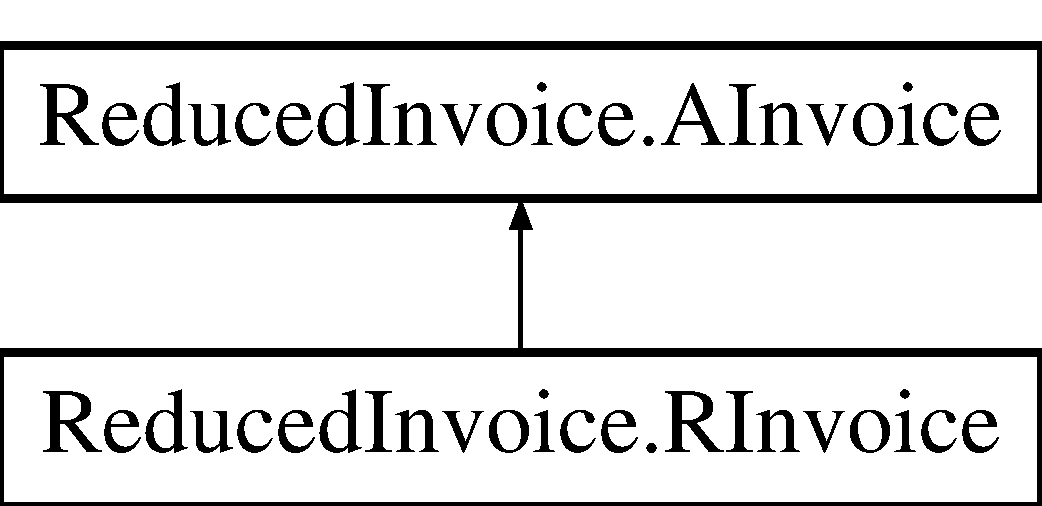
\includegraphics[height=2.000000cm]{class_reduced_invoice_1_1_a_invoice}
\end{center}
\end{figure}
\subsection*{Classes}
\begin{DoxyCompactItemize}
\item 
enum \hyperlink{enum_reduced_invoice_1_1_a_invoice_1_1_error}{Error}
\end{DoxyCompactItemize}
\subsection*{Public Member Functions}
\begin{DoxyCompactItemize}
\item 
String \hyperlink{class_reduced_invoice_1_1_a_invoice_a0099d82cccbb09bc9240269c76c079d4}{get\+Buyer\+Name} ()
\item 
void \hyperlink{class_reduced_invoice_1_1_a_invoice_ab47710855319e2cf64a829d9bb37d243}{set\+Buyer\+Name} (String \hyperlink{class_reduced_invoice_1_1_a_invoice_ae75bdd20da8fa21dec01c2d032ac11c5}{buyer\+Name})
\item 
String \hyperlink{class_reduced_invoice_1_1_a_invoice_ac8973df8a999bc5556d697ed17c871f7}{get\+Seller\+Name} ()
\item 
void \hyperlink{class_reduced_invoice_1_1_a_invoice_a45129f98801ec280c52c2de35b48da0b}{set\+Seller\+Name} (String \hyperlink{class_reduced_invoice_1_1_a_invoice_ae00a97e1c74841fe0b0b43fccd1da24d}{seller\+Name})
\item 
abstract void \hyperlink{class_reduced_invoice_1_1_a_invoice_a29b30209d39ee91edee303ba5d36fd81}{add\+Position} (\hyperlink{class_reduced_invoice_1_1_position}{Position} p)
\item 
abstract void \hyperlink{class_reduced_invoice_1_1_a_invoice_ae126e009135936362d30c61ea7b20b52}{add\+Position} (String desc, \hyperlink{class_reduced_invoice_1_1_price}{Price} p, String mm, int amount, int tax)
\item 
abstract void \hyperlink{class_reduced_invoice_1_1_a_invoice_a0ccc4c6c378676635b552e12c6a7d690}{add\+Position} (String desc, \hyperlink{class_reduced_invoice_1_1_price}{Price} p, String mm, int amount, int tax, \hyperlink{enum_reduced_invoice_1_1_a_invoice_1_1_error}{Error} positionerror)
\item 
abstract \hyperlink{class_reduced_invoice_1_1_position}{Position} \hyperlink{class_reduced_invoice_1_1_a_invoice_a1264648436c734afc549b2d1adb20ff6}{get\+Position} (int index)
\item 
abstract List$<$ \hyperlink{class_reduced_invoice_1_1_position}{Position} $>$ \hyperlink{class_reduced_invoice_1_1_a_invoice_a62a407f4bec81c5dbd392f68ecff6582}{get\+Positions} ()
\item 
abstract void \hyperlink{class_reduced_invoice_1_1_a_invoice_a3abfa40d89bdc9f56daaf73adafcca5e}{set\+Position} (\hyperlink{class_reduced_invoice_1_1_position}{Position} position, int index)
\item 
abstract void \hyperlink{class_reduced_invoice_1_1_a_invoice_a01a6d1c001117851fdcb6941a117c086}{set\+Position\+Description} (String description, int index)
\item 
abstract void \hyperlink{class_reduced_invoice_1_1_a_invoice_a0fb3b8175eac0e76c906a986ba7d6161}{set\+Position\+Price} (\hyperlink{class_reduced_invoice_1_1_price}{Price} price, int index)
\item 
abstract void \hyperlink{class_reduced_invoice_1_1_a_invoice_aef6af27bf12024c16e8e5890243825eb}{set\+Position\+Amount} (int amount, int index)
\item 
abstract void \hyperlink{class_reduced_invoice_1_1_a_invoice_a5919a1c5d917fc62d654441f582f470e}{set\+Position\+Tax\+Rate} (int taxrate, int index)
\item 
abstract int \hyperlink{class_reduced_invoice_1_1_a_invoice_a109ff7a484de183356ebe38737556f11}{get\+Positions\+Length} ()
\item 
String \hyperlink{class_reduced_invoice_1_1_a_invoice_ae420c9c0e825a538be46f1fce2c18c57}{get\+Voucher\+ID} ()
\item 
void \hyperlink{class_reduced_invoice_1_1_a_invoice_a042790fb1b2c097d0da994c255fa9dc4}{set\+Voucher\+ID} (String Voucher\+ID)
\item 
Date \hyperlink{class_reduced_invoice_1_1_a_invoice_ac78ce56c3ae003ca87e8144546d7ec3f}{get\+Invoice\+Date} ()
\item 
void \hyperlink{class_reduced_invoice_1_1_a_invoice_adefa18f4aec87c1d4b89233baf6ce9ee}{set\+Invoice\+Date} (Date invoice\+Date)
\item 
String \hyperlink{class_reduced_invoice_1_1_a_invoice_a09231d505794762ea8f363e4689392c8}{get\+Invoice\+Number} ()
\item 
void \hyperlink{class_reduced_invoice_1_1_a_invoice_a20d784a1da556e7bb3c5538c5a6701c4}{set\+Invoice\+Number} (String invoice\+Number)
\item 
String \hyperlink{class_reduced_invoice_1_1_a_invoice_a2c0175f8fdd6c21504bdf6f8e3336cc2}{get\+Currency} ()
\item 
void \hyperlink{class_reduced_invoice_1_1_a_invoice_a83a6ba629194d28ea32c24275d0e14ba}{set\+Currency} (String currency)
\item 
\hyperlink{class_reduced_invoice_1_1_price}{Price} \hyperlink{class_reduced_invoice_1_1_a_invoice_aedc84169ce345d6f7c72b808c305c27b}{get\+Total\+Price} ()
\item 
void \hyperlink{class_reduced_invoice_1_1_a_invoice_ac5c395d78cb3bd54e8e40678bdb46bf0}{set\+Total\+Price} (\hyperlink{class_reduced_invoice_1_1_price}{Price} total\+Price)
\item 
\hyperlink{enum_reduced_invoice_1_1_a_invoice_1_1_error}{Error} \hyperlink{class_reduced_invoice_1_1_a_invoice_ac6335f5b80ba3514a205e46c7170ae5c}{get\+Invoice\+Error} ()
\item 
void \hyperlink{class_reduced_invoice_1_1_a_invoice_a625c87b0ecdcbf896e66e4ad1fe31681}{set\+Invoice\+Error} (\hyperlink{enum_reduced_invoice_1_1_a_invoice_1_1_error}{Error} invoiceerror)
\item 
void \hyperlink{class_reduced_invoice_1_1_a_invoice_ae629ee52330ced3e2e3865159591b6bf}{set\+Invoice\+Error\+\_\+\+V\+O\+U\+C\+H\+E\+R\+\_\+\+I\+D\+\_\+\+E\+R\+R\+OR} ()
\item 
void \hyperlink{class_reduced_invoice_1_1_a_invoice_a84d5f81b1ad887324d38d2cd13e1fded}{set\+Invoice\+Error\+\_\+\+R\+E\+C\+O\+N\+S\+T\+R\+U\+C\+T\+\_\+\+E\+R\+R\+OR} ()
\item 
boolean \hyperlink{class_reduced_invoice_1_1_a_invoice_ad1cf29d7670fe6dc9410c41cb7c676de}{check\+Voucher\+I\+D\+Error} ()
\item 
boolean \hyperlink{class_reduced_invoice_1_1_a_invoice_a010f92b723472fce5b2885530e68329e}{check\+Reconstruct\+Voucher\+Error} ()
\item 
\hyperlink{class_reduced_invoice_1_1_metadata}{Metadata} \hyperlink{class_reduced_invoice_1_1_a_invoice_a27064d52b653a15a81485e72b54fd687}{get\+Meta\+Data} ()
\item 
void \hyperlink{class_reduced_invoice_1_1_a_invoice_a67f0ef58970f9aff38098d079e738596}{set\+Meta\+Data} (\hyperlink{class_reduced_invoice_1_1_metadata}{Metadata} meta\+Data)
\end{DoxyCompactItemize}
\subsection*{Protected Attributes}
\begin{DoxyCompactItemize}
\item 
String \hyperlink{class_reduced_invoice_1_1_a_invoice_ae75bdd20da8fa21dec01c2d032ac11c5}{buyer\+Name}
\item 
String \hyperlink{class_reduced_invoice_1_1_a_invoice_ae00a97e1c74841fe0b0b43fccd1da24d}{seller\+Name}
\item 
\hyperlink{class_reduced_invoice_1_1_price}{Price} \hyperlink{class_reduced_invoice_1_1_a_invoice_a72b831e7ee0b4501fc949f61aecdd498}{Total\+Price}
\item 
List$<$ \hyperlink{class_reduced_invoice_1_1_position}{Position} $>$ \hyperlink{class_reduced_invoice_1_1_a_invoice_a5b51f1865386bd021580507c7133f69a}{Positions}
\item 
String \hyperlink{class_reduced_invoice_1_1_a_invoice_a6b6ef26c85bc07f70cb7b4c8eb057fe8}{Currency}
\item 
\hyperlink{enum_reduced_invoice_1_1_a_invoice_1_1_error}{Error} \hyperlink{class_reduced_invoice_1_1_a_invoice_a3ef6a3a4efa7e9b652f5399bc76e017a}{Invoice\+Error}
\end{DoxyCompactItemize}


\subsection{Detailed Description}


Definition at line 6 of file A\+Invoice.\+java.



\subsection{Member Function Documentation}
\index{Reduced\+Invoice\+::\+A\+Invoice@{Reduced\+Invoice\+::\+A\+Invoice}!add\+Position@{add\+Position}}
\index{add\+Position@{add\+Position}!Reduced\+Invoice\+::\+A\+Invoice@{Reduced\+Invoice\+::\+A\+Invoice}}
\subsubsection[{\texorpdfstring{add\+Position(\+Position p)}{addPosition(Position p)}}]{\setlength{\rightskip}{0pt plus 5cm}abstract void Reduced\+Invoice.\+A\+Invoice.\+add\+Position (
\begin{DoxyParamCaption}
\item[{{\bf Position}}]{p}
\end{DoxyParamCaption}
)\hspace{0.3cm}{\ttfamily [abstract]}}\hypertarget{class_reduced_invoice_1_1_a_invoice_a29b30209d39ee91edee303ba5d36fd81}{}\label{class_reduced_invoice_1_1_a_invoice_a29b30209d39ee91edee303ba5d36fd81}
\index{Reduced\+Invoice\+::\+A\+Invoice@{Reduced\+Invoice\+::\+A\+Invoice}!add\+Position@{add\+Position}}
\index{add\+Position@{add\+Position}!Reduced\+Invoice\+::\+A\+Invoice@{Reduced\+Invoice\+::\+A\+Invoice}}
\subsubsection[{\texorpdfstring{add\+Position(\+String desc, Price p, String mm, int amount, int tax)}{addPosition(String desc, Price p, String mm, int amount, int tax)}}]{\setlength{\rightskip}{0pt plus 5cm}abstract void Reduced\+Invoice.\+A\+Invoice.\+add\+Position (
\begin{DoxyParamCaption}
\item[{String}]{desc, }
\item[{{\bf Price}}]{p, }
\item[{String}]{mm, }
\item[{int}]{amount, }
\item[{int}]{tax}
\end{DoxyParamCaption}
)\hspace{0.3cm}{\ttfamily [abstract]}}\hypertarget{class_reduced_invoice_1_1_a_invoice_ae126e009135936362d30c61ea7b20b52}{}\label{class_reduced_invoice_1_1_a_invoice_ae126e009135936362d30c61ea7b20b52}
\index{Reduced\+Invoice\+::\+A\+Invoice@{Reduced\+Invoice\+::\+A\+Invoice}!add\+Position@{add\+Position}}
\index{add\+Position@{add\+Position}!Reduced\+Invoice\+::\+A\+Invoice@{Reduced\+Invoice\+::\+A\+Invoice}}
\subsubsection[{\texorpdfstring{add\+Position(\+String desc, Price p, String mm, int amount, int tax, Error positionerror)}{addPosition(String desc, Price p, String mm, int amount, int tax, Error positionerror)}}]{\setlength{\rightskip}{0pt plus 5cm}abstract void Reduced\+Invoice.\+A\+Invoice.\+add\+Position (
\begin{DoxyParamCaption}
\item[{String}]{desc, }
\item[{{\bf Price}}]{p, }
\item[{String}]{mm, }
\item[{int}]{amount, }
\item[{int}]{tax, }
\item[{{\bf Error}}]{positionerror}
\end{DoxyParamCaption}
)\hspace{0.3cm}{\ttfamily [abstract]}}\hypertarget{class_reduced_invoice_1_1_a_invoice_a0ccc4c6c378676635b552e12c6a7d690}{}\label{class_reduced_invoice_1_1_a_invoice_a0ccc4c6c378676635b552e12c6a7d690}
\index{Reduced\+Invoice\+::\+A\+Invoice@{Reduced\+Invoice\+::\+A\+Invoice}!check\+Reconstruct\+Voucher\+Error@{check\+Reconstruct\+Voucher\+Error}}
\index{check\+Reconstruct\+Voucher\+Error@{check\+Reconstruct\+Voucher\+Error}!Reduced\+Invoice\+::\+A\+Invoice@{Reduced\+Invoice\+::\+A\+Invoice}}
\subsubsection[{\texorpdfstring{check\+Reconstruct\+Voucher\+Error()}{checkReconstructVoucherError()}}]{\setlength{\rightskip}{0pt plus 5cm}boolean Reduced\+Invoice.\+A\+Invoice.\+check\+Reconstruct\+Voucher\+Error (
\begin{DoxyParamCaption}
{}
\end{DoxyParamCaption}
)\hspace{0.3cm}{\ttfamily [inline]}}\hypertarget{class_reduced_invoice_1_1_a_invoice_a010f92b723472fce5b2885530e68329e}{}\label{class_reduced_invoice_1_1_a_invoice_a010f92b723472fce5b2885530e68329e}


Definition at line 150 of file A\+Invoice.\+java.


\begin{DoxyCode}
151     \{
152         \textcolor{keywordflow}{if}(\hyperlink{class_reduced_invoice_1_1_a_invoice_a3ef6a3a4efa7e9b652f5399bc76e017a}{InvoiceError} == Error.\hyperlink{enum_reduced_invoice_1_1_a_invoice_1_1_error_af28e1c7484bcb6f47f70a00e9dd81671}{RECONSTRUCT\_ERROR})
153             \textcolor{keywordflow}{return} \textcolor{keyword}{true};
154         \textcolor{keywordflow}{else}
155             \textcolor{keywordflow}{return} \textcolor{keyword}{false};
156     \}
\end{DoxyCode}
\index{Reduced\+Invoice\+::\+A\+Invoice@{Reduced\+Invoice\+::\+A\+Invoice}!check\+Voucher\+I\+D\+Error@{check\+Voucher\+I\+D\+Error}}
\index{check\+Voucher\+I\+D\+Error@{check\+Voucher\+I\+D\+Error}!Reduced\+Invoice\+::\+A\+Invoice@{Reduced\+Invoice\+::\+A\+Invoice}}
\subsubsection[{\texorpdfstring{check\+Voucher\+I\+D\+Error()}{checkVoucherIDError()}}]{\setlength{\rightskip}{0pt plus 5cm}boolean Reduced\+Invoice.\+A\+Invoice.\+check\+Voucher\+I\+D\+Error (
\begin{DoxyParamCaption}
{}
\end{DoxyParamCaption}
)\hspace{0.3cm}{\ttfamily [inline]}}\hypertarget{class_reduced_invoice_1_1_a_invoice_ad1cf29d7670fe6dc9410c41cb7c676de}{}\label{class_reduced_invoice_1_1_a_invoice_ad1cf29d7670fe6dc9410c41cb7c676de}


Definition at line 142 of file A\+Invoice.\+java.


\begin{DoxyCode}
143     \{
144         \textcolor{keywordflow}{if}(\hyperlink{class_reduced_invoice_1_1_a_invoice_a3ef6a3a4efa7e9b652f5399bc76e017a}{InvoiceError} == Error.\hyperlink{enum_reduced_invoice_1_1_a_invoice_1_1_error_aac88b1b92765c5fdea043f9c9aeeb701}{VOUCHER\_ID\_ERROR})
145             \textcolor{keywordflow}{return} \textcolor{keyword}{true};
146         \textcolor{keywordflow}{else}
147             \textcolor{keywordflow}{return} \textcolor{keyword}{false};
148     \}
\end{DoxyCode}
\index{Reduced\+Invoice\+::\+A\+Invoice@{Reduced\+Invoice\+::\+A\+Invoice}!get\+Buyer\+Name@{get\+Buyer\+Name}}
\index{get\+Buyer\+Name@{get\+Buyer\+Name}!Reduced\+Invoice\+::\+A\+Invoice@{Reduced\+Invoice\+::\+A\+Invoice}}
\subsubsection[{\texorpdfstring{get\+Buyer\+Name()}{getBuyerName()}}]{\setlength{\rightskip}{0pt plus 5cm}String Reduced\+Invoice.\+A\+Invoice.\+get\+Buyer\+Name (
\begin{DoxyParamCaption}
{}
\end{DoxyParamCaption}
)\hspace{0.3cm}{\ttfamily [inline]}}\hypertarget{class_reduced_invoice_1_1_a_invoice_a0099d82cccbb09bc9240269c76c079d4}{}\label{class_reduced_invoice_1_1_a_invoice_a0099d82cccbb09bc9240269c76c079d4}


Definition at line 38 of file A\+Invoice.\+java.


\begin{DoxyCode}
38                                  \{
39         \textcolor{keywordflow}{return} \hyperlink{class_reduced_invoice_1_1_a_invoice_ae75bdd20da8fa21dec01c2d032ac11c5}{buyerName};
40     \}
\end{DoxyCode}
\index{Reduced\+Invoice\+::\+A\+Invoice@{Reduced\+Invoice\+::\+A\+Invoice}!get\+Currency@{get\+Currency}}
\index{get\+Currency@{get\+Currency}!Reduced\+Invoice\+::\+A\+Invoice@{Reduced\+Invoice\+::\+A\+Invoice}}
\subsubsection[{\texorpdfstring{get\+Currency()}{getCurrency()}}]{\setlength{\rightskip}{0pt plus 5cm}String Reduced\+Invoice.\+A\+Invoice.\+get\+Currency (
\begin{DoxyParamCaption}
{}
\end{DoxyParamCaption}
)\hspace{0.3cm}{\ttfamily [inline]}}\hypertarget{class_reduced_invoice_1_1_a_invoice_a2c0175f8fdd6c21504bdf6f8e3336cc2}{}\label{class_reduced_invoice_1_1_a_invoice_a2c0175f8fdd6c21504bdf6f8e3336cc2}


Definition at line 103 of file A\+Invoice.\+java.


\begin{DoxyCode}
103                                 \{
104         \textcolor{keywordflow}{return} \hyperlink{class_reduced_invoice_1_1_a_invoice_a6b6ef26c85bc07f70cb7b4c8eb057fe8}{Currency};
105     \}
\end{DoxyCode}
\index{Reduced\+Invoice\+::\+A\+Invoice@{Reduced\+Invoice\+::\+A\+Invoice}!get\+Invoice\+Date@{get\+Invoice\+Date}}
\index{get\+Invoice\+Date@{get\+Invoice\+Date}!Reduced\+Invoice\+::\+A\+Invoice@{Reduced\+Invoice\+::\+A\+Invoice}}
\subsubsection[{\texorpdfstring{get\+Invoice\+Date()}{getInvoiceDate()}}]{\setlength{\rightskip}{0pt plus 5cm}Date Reduced\+Invoice.\+A\+Invoice.\+get\+Invoice\+Date (
\begin{DoxyParamCaption}
{}
\end{DoxyParamCaption}
)\hspace{0.3cm}{\ttfamily [inline]}}\hypertarget{class_reduced_invoice_1_1_a_invoice_ac78ce56c3ae003ca87e8144546d7ec3f}{}\label{class_reduced_invoice_1_1_a_invoice_ac78ce56c3ae003ca87e8144546d7ec3f}


Definition at line 86 of file A\+Invoice.\+java.


\begin{DoxyCode}
86                                  \{
87         \textcolor{keywordflow}{return} invoiceDate;
88     \}
\end{DoxyCode}
\index{Reduced\+Invoice\+::\+A\+Invoice@{Reduced\+Invoice\+::\+A\+Invoice}!get\+Invoice\+Error@{get\+Invoice\+Error}}
\index{get\+Invoice\+Error@{get\+Invoice\+Error}!Reduced\+Invoice\+::\+A\+Invoice@{Reduced\+Invoice\+::\+A\+Invoice}}
\subsubsection[{\texorpdfstring{get\+Invoice\+Error()}{getInvoiceError()}}]{\setlength{\rightskip}{0pt plus 5cm}{\bf Error} Reduced\+Invoice.\+A\+Invoice.\+get\+Invoice\+Error (
\begin{DoxyParamCaption}
{}
\end{DoxyParamCaption}
)\hspace{0.3cm}{\ttfamily [inline]}}\hypertarget{class_reduced_invoice_1_1_a_invoice_ac6335f5b80ba3514a205e46c7170ae5c}{}\label{class_reduced_invoice_1_1_a_invoice_ac6335f5b80ba3514a205e46c7170ae5c}


Definition at line 122 of file A\+Invoice.\+java.


\begin{DoxyCode}
123     \{
124         \textcolor{keywordflow}{return} \hyperlink{class_reduced_invoice_1_1_a_invoice_a3ef6a3a4efa7e9b652f5399bc76e017a}{InvoiceError};
125     \}
\end{DoxyCode}
\index{Reduced\+Invoice\+::\+A\+Invoice@{Reduced\+Invoice\+::\+A\+Invoice}!get\+Invoice\+Number@{get\+Invoice\+Number}}
\index{get\+Invoice\+Number@{get\+Invoice\+Number}!Reduced\+Invoice\+::\+A\+Invoice@{Reduced\+Invoice\+::\+A\+Invoice}}
\subsubsection[{\texorpdfstring{get\+Invoice\+Number()}{getInvoiceNumber()}}]{\setlength{\rightskip}{0pt plus 5cm}String Reduced\+Invoice.\+A\+Invoice.\+get\+Invoice\+Number (
\begin{DoxyParamCaption}
{}
\end{DoxyParamCaption}
)\hspace{0.3cm}{\ttfamily [inline]}}\hypertarget{class_reduced_invoice_1_1_a_invoice_a09231d505794762ea8f363e4689392c8}{}\label{class_reduced_invoice_1_1_a_invoice_a09231d505794762ea8f363e4689392c8}


Definition at line 94 of file A\+Invoice.\+java.


\begin{DoxyCode}
94                                      \{
95         \textcolor{keywordflow}{return} invoiceNumber;
96     \}
\end{DoxyCode}
\index{Reduced\+Invoice\+::\+A\+Invoice@{Reduced\+Invoice\+::\+A\+Invoice}!get\+Meta\+Data@{get\+Meta\+Data}}
\index{get\+Meta\+Data@{get\+Meta\+Data}!Reduced\+Invoice\+::\+A\+Invoice@{Reduced\+Invoice\+::\+A\+Invoice}}
\subsubsection[{\texorpdfstring{get\+Meta\+Data()}{getMetaData()}}]{\setlength{\rightskip}{0pt plus 5cm}{\bf Metadata} Reduced\+Invoice.\+A\+Invoice.\+get\+Meta\+Data (
\begin{DoxyParamCaption}
{}
\end{DoxyParamCaption}
)\hspace{0.3cm}{\ttfamily [inline]}}\hypertarget{class_reduced_invoice_1_1_a_invoice_a27064d52b653a15a81485e72b54fd687}{}\label{class_reduced_invoice_1_1_a_invoice_a27064d52b653a15a81485e72b54fd687}


Definition at line 158 of file A\+Invoice.\+java.


\begin{DoxyCode}
158                                   \{
159         \textcolor{keywordflow}{return} MetaData;
160     \}
\end{DoxyCode}
\index{Reduced\+Invoice\+::\+A\+Invoice@{Reduced\+Invoice\+::\+A\+Invoice}!get\+Position@{get\+Position}}
\index{get\+Position@{get\+Position}!Reduced\+Invoice\+::\+A\+Invoice@{Reduced\+Invoice\+::\+A\+Invoice}}
\subsubsection[{\texorpdfstring{get\+Position(int index)}{getPosition(int index)}}]{\setlength{\rightskip}{0pt plus 5cm}abstract {\bf Position} Reduced\+Invoice.\+A\+Invoice.\+get\+Position (
\begin{DoxyParamCaption}
\item[{int}]{index}
\end{DoxyParamCaption}
)\hspace{0.3cm}{\ttfamily [abstract]}}\hypertarget{class_reduced_invoice_1_1_a_invoice_a1264648436c734afc549b2d1adb20ff6}{}\label{class_reduced_invoice_1_1_a_invoice_a1264648436c734afc549b2d1adb20ff6}
\index{Reduced\+Invoice\+::\+A\+Invoice@{Reduced\+Invoice\+::\+A\+Invoice}!get\+Positions@{get\+Positions}}
\index{get\+Positions@{get\+Positions}!Reduced\+Invoice\+::\+A\+Invoice@{Reduced\+Invoice\+::\+A\+Invoice}}
\subsubsection[{\texorpdfstring{get\+Positions()}{getPositions()}}]{\setlength{\rightskip}{0pt plus 5cm}abstract List$<${\bf Position}$>$ Reduced\+Invoice.\+A\+Invoice.\+get\+Positions (
\begin{DoxyParamCaption}
{}
\end{DoxyParamCaption}
)\hspace{0.3cm}{\ttfamily [abstract]}}\hypertarget{class_reduced_invoice_1_1_a_invoice_a62a407f4bec81c5dbd392f68ecff6582}{}\label{class_reduced_invoice_1_1_a_invoice_a62a407f4bec81c5dbd392f68ecff6582}
\index{Reduced\+Invoice\+::\+A\+Invoice@{Reduced\+Invoice\+::\+A\+Invoice}!get\+Positions\+Length@{get\+Positions\+Length}}
\index{get\+Positions\+Length@{get\+Positions\+Length}!Reduced\+Invoice\+::\+A\+Invoice@{Reduced\+Invoice\+::\+A\+Invoice}}
\subsubsection[{\texorpdfstring{get\+Positions\+Length()}{getPositionsLength()}}]{\setlength{\rightskip}{0pt plus 5cm}abstract int Reduced\+Invoice.\+A\+Invoice.\+get\+Positions\+Length (
\begin{DoxyParamCaption}
{}
\end{DoxyParamCaption}
)\hspace{0.3cm}{\ttfamily [abstract]}}\hypertarget{class_reduced_invoice_1_1_a_invoice_a109ff7a484de183356ebe38737556f11}{}\label{class_reduced_invoice_1_1_a_invoice_a109ff7a484de183356ebe38737556f11}
\index{Reduced\+Invoice\+::\+A\+Invoice@{Reduced\+Invoice\+::\+A\+Invoice}!get\+Seller\+Name@{get\+Seller\+Name}}
\index{get\+Seller\+Name@{get\+Seller\+Name}!Reduced\+Invoice\+::\+A\+Invoice@{Reduced\+Invoice\+::\+A\+Invoice}}
\subsubsection[{\texorpdfstring{get\+Seller\+Name()}{getSellerName()}}]{\setlength{\rightskip}{0pt plus 5cm}String Reduced\+Invoice.\+A\+Invoice.\+get\+Seller\+Name (
\begin{DoxyParamCaption}
{}
\end{DoxyParamCaption}
)\hspace{0.3cm}{\ttfamily [inline]}}\hypertarget{class_reduced_invoice_1_1_a_invoice_ac8973df8a999bc5556d697ed17c871f7}{}\label{class_reduced_invoice_1_1_a_invoice_ac8973df8a999bc5556d697ed17c871f7}


Definition at line 46 of file A\+Invoice.\+java.


\begin{DoxyCode}
46                                   \{
47         \textcolor{keywordflow}{return} \hyperlink{class_reduced_invoice_1_1_a_invoice_ae00a97e1c74841fe0b0b43fccd1da24d}{sellerName};
48     \}
\end{DoxyCode}
\index{Reduced\+Invoice\+::\+A\+Invoice@{Reduced\+Invoice\+::\+A\+Invoice}!get\+Total\+Price@{get\+Total\+Price}}
\index{get\+Total\+Price@{get\+Total\+Price}!Reduced\+Invoice\+::\+A\+Invoice@{Reduced\+Invoice\+::\+A\+Invoice}}
\subsubsection[{\texorpdfstring{get\+Total\+Price()}{getTotalPrice()}}]{\setlength{\rightskip}{0pt plus 5cm}{\bf Price} Reduced\+Invoice.\+A\+Invoice.\+get\+Total\+Price (
\begin{DoxyParamCaption}
{}
\end{DoxyParamCaption}
)\hspace{0.3cm}{\ttfamily [inline]}}\hypertarget{class_reduced_invoice_1_1_a_invoice_aedc84169ce345d6f7c72b808c305c27b}{}\label{class_reduced_invoice_1_1_a_invoice_aedc84169ce345d6f7c72b808c305c27b}


Definition at line 113 of file A\+Invoice.\+java.


\begin{DoxyCode}
113                                  \{
114         \textcolor{keywordflow}{return} \hyperlink{class_reduced_invoice_1_1_a_invoice_a72b831e7ee0b4501fc949f61aecdd498}{TotalPrice};
115     \}
\end{DoxyCode}
\index{Reduced\+Invoice\+::\+A\+Invoice@{Reduced\+Invoice\+::\+A\+Invoice}!get\+Voucher\+ID@{get\+Voucher\+ID}}
\index{get\+Voucher\+ID@{get\+Voucher\+ID}!Reduced\+Invoice\+::\+A\+Invoice@{Reduced\+Invoice\+::\+A\+Invoice}}
\subsubsection[{\texorpdfstring{get\+Voucher\+I\+D()}{getVoucherID()}}]{\setlength{\rightskip}{0pt plus 5cm}String Reduced\+Invoice.\+A\+Invoice.\+get\+Voucher\+ID (
\begin{DoxyParamCaption}
{}
\end{DoxyParamCaption}
)\hspace{0.3cm}{\ttfamily [inline]}}\hypertarget{class_reduced_invoice_1_1_a_invoice_ae420c9c0e825a538be46f1fce2c18c57}{}\label{class_reduced_invoice_1_1_a_invoice_ae420c9c0e825a538be46f1fce2c18c57}


Definition at line 76 of file A\+Invoice.\+java.


\begin{DoxyCode}
77     \{
78         \textcolor{keywordflow}{return} VoucherID;
79     \}
\end{DoxyCode}
\index{Reduced\+Invoice\+::\+A\+Invoice@{Reduced\+Invoice\+::\+A\+Invoice}!set\+Buyer\+Name@{set\+Buyer\+Name}}
\index{set\+Buyer\+Name@{set\+Buyer\+Name}!Reduced\+Invoice\+::\+A\+Invoice@{Reduced\+Invoice\+::\+A\+Invoice}}
\subsubsection[{\texorpdfstring{set\+Buyer\+Name(\+String buyer\+Name)}{setBuyerName(String buyerName)}}]{\setlength{\rightskip}{0pt plus 5cm}void Reduced\+Invoice.\+A\+Invoice.\+set\+Buyer\+Name (
\begin{DoxyParamCaption}
\item[{String}]{buyer\+Name}
\end{DoxyParamCaption}
)\hspace{0.3cm}{\ttfamily [inline]}}\hypertarget{class_reduced_invoice_1_1_a_invoice_ab47710855319e2cf64a829d9bb37d243}{}\label{class_reduced_invoice_1_1_a_invoice_ab47710855319e2cf64a829d9bb37d243}


Definition at line 42 of file A\+Invoice.\+java.


\begin{DoxyCode}
42                                                \{
43         this.\hyperlink{class_reduced_invoice_1_1_a_invoice_ae75bdd20da8fa21dec01c2d032ac11c5}{buyerName} = \hyperlink{class_reduced_invoice_1_1_a_invoice_ae75bdd20da8fa21dec01c2d032ac11c5}{buyerName};
44     \}
\end{DoxyCode}
\index{Reduced\+Invoice\+::\+A\+Invoice@{Reduced\+Invoice\+::\+A\+Invoice}!set\+Currency@{set\+Currency}}
\index{set\+Currency@{set\+Currency}!Reduced\+Invoice\+::\+A\+Invoice@{Reduced\+Invoice\+::\+A\+Invoice}}
\subsubsection[{\texorpdfstring{set\+Currency(\+String currency)}{setCurrency(String currency)}}]{\setlength{\rightskip}{0pt plus 5cm}void Reduced\+Invoice.\+A\+Invoice.\+set\+Currency (
\begin{DoxyParamCaption}
\item[{String}]{currency}
\end{DoxyParamCaption}
)\hspace{0.3cm}{\ttfamily [inline]}}\hypertarget{class_reduced_invoice_1_1_a_invoice_a83a6ba629194d28ea32c24275d0e14ba}{}\label{class_reduced_invoice_1_1_a_invoice_a83a6ba629194d28ea32c24275d0e14ba}


Definition at line 108 of file A\+Invoice.\+java.


\begin{DoxyCode}
108                                              \{
109         \hyperlink{class_reduced_invoice_1_1_a_invoice_a6b6ef26c85bc07f70cb7b4c8eb057fe8}{Currency} = currency;
110     \}
\end{DoxyCode}
\index{Reduced\+Invoice\+::\+A\+Invoice@{Reduced\+Invoice\+::\+A\+Invoice}!set\+Invoice\+Date@{set\+Invoice\+Date}}
\index{set\+Invoice\+Date@{set\+Invoice\+Date}!Reduced\+Invoice\+::\+A\+Invoice@{Reduced\+Invoice\+::\+A\+Invoice}}
\subsubsection[{\texorpdfstring{set\+Invoice\+Date(\+Date invoice\+Date)}{setInvoiceDate(Date invoiceDate)}}]{\setlength{\rightskip}{0pt plus 5cm}void Reduced\+Invoice.\+A\+Invoice.\+set\+Invoice\+Date (
\begin{DoxyParamCaption}
\item[{Date}]{invoice\+Date}
\end{DoxyParamCaption}
)\hspace{0.3cm}{\ttfamily [inline]}}\hypertarget{class_reduced_invoice_1_1_a_invoice_adefa18f4aec87c1d4b89233baf6ce9ee}{}\label{class_reduced_invoice_1_1_a_invoice_adefa18f4aec87c1d4b89233baf6ce9ee}


Definition at line 90 of file A\+Invoice.\+java.


\begin{DoxyCode}
90                                                  \{
91         this.invoiceDate = invoiceDate;
92     \}
\end{DoxyCode}
\index{Reduced\+Invoice\+::\+A\+Invoice@{Reduced\+Invoice\+::\+A\+Invoice}!set\+Invoice\+Error@{set\+Invoice\+Error}}
\index{set\+Invoice\+Error@{set\+Invoice\+Error}!Reduced\+Invoice\+::\+A\+Invoice@{Reduced\+Invoice\+::\+A\+Invoice}}
\subsubsection[{\texorpdfstring{set\+Invoice\+Error(\+Error invoiceerror)}{setInvoiceError(Error invoiceerror)}}]{\setlength{\rightskip}{0pt plus 5cm}void Reduced\+Invoice.\+A\+Invoice.\+set\+Invoice\+Error (
\begin{DoxyParamCaption}
\item[{{\bf Error}}]{invoiceerror}
\end{DoxyParamCaption}
)\hspace{0.3cm}{\ttfamily [inline]}}\hypertarget{class_reduced_invoice_1_1_a_invoice_a625c87b0ecdcbf896e66e4ad1fe31681}{}\label{class_reduced_invoice_1_1_a_invoice_a625c87b0ecdcbf896e66e4ad1fe31681}


Definition at line 127 of file A\+Invoice.\+java.


\begin{DoxyCode}
128     \{
129         \hyperlink{class_reduced_invoice_1_1_a_invoice_a3ef6a3a4efa7e9b652f5399bc76e017a}{InvoiceError} = invoiceerror;
130     \}
\end{DoxyCode}
\index{Reduced\+Invoice\+::\+A\+Invoice@{Reduced\+Invoice\+::\+A\+Invoice}!set\+Invoice\+Error\+\_\+\+R\+E\+C\+O\+N\+S\+T\+R\+U\+C\+T\+\_\+\+E\+R\+R\+OR@{set\+Invoice\+Error\+\_\+\+R\+E\+C\+O\+N\+S\+T\+R\+U\+C\+T\+\_\+\+E\+R\+R\+OR}}
\index{set\+Invoice\+Error\+\_\+\+R\+E\+C\+O\+N\+S\+T\+R\+U\+C\+T\+\_\+\+E\+R\+R\+OR@{set\+Invoice\+Error\+\_\+\+R\+E\+C\+O\+N\+S\+T\+R\+U\+C\+T\+\_\+\+E\+R\+R\+OR}!Reduced\+Invoice\+::\+A\+Invoice@{Reduced\+Invoice\+::\+A\+Invoice}}
\subsubsection[{\texorpdfstring{set\+Invoice\+Error\+\_\+\+R\+E\+C\+O\+N\+S\+T\+R\+U\+C\+T\+\_\+\+E\+R\+R\+O\+R()}{setInvoiceError_RECONSTRUCT_ERROR()}}]{\setlength{\rightskip}{0pt plus 5cm}void Reduced\+Invoice.\+A\+Invoice.\+set\+Invoice\+Error\+\_\+\+R\+E\+C\+O\+N\+S\+T\+R\+U\+C\+T\+\_\+\+E\+R\+R\+OR (
\begin{DoxyParamCaption}
{}
\end{DoxyParamCaption}
)\hspace{0.3cm}{\ttfamily [inline]}}\hypertarget{class_reduced_invoice_1_1_a_invoice_a84d5f81b1ad887324d38d2cd13e1fded}{}\label{class_reduced_invoice_1_1_a_invoice_a84d5f81b1ad887324d38d2cd13e1fded}


Definition at line 137 of file A\+Invoice.\+java.


\begin{DoxyCode}
138     \{
139         \hyperlink{class_reduced_invoice_1_1_a_invoice_a3ef6a3a4efa7e9b652f5399bc76e017a}{InvoiceError} = Error.\hyperlink{enum_reduced_invoice_1_1_a_invoice_1_1_error_af28e1c7484bcb6f47f70a00e9dd81671}{RECONSTRUCT\_ERROR};
140     \}
\end{DoxyCode}
\index{Reduced\+Invoice\+::\+A\+Invoice@{Reduced\+Invoice\+::\+A\+Invoice}!set\+Invoice\+Error\+\_\+\+V\+O\+U\+C\+H\+E\+R\+\_\+\+I\+D\+\_\+\+E\+R\+R\+OR@{set\+Invoice\+Error\+\_\+\+V\+O\+U\+C\+H\+E\+R\+\_\+\+I\+D\+\_\+\+E\+R\+R\+OR}}
\index{set\+Invoice\+Error\+\_\+\+V\+O\+U\+C\+H\+E\+R\+\_\+\+I\+D\+\_\+\+E\+R\+R\+OR@{set\+Invoice\+Error\+\_\+\+V\+O\+U\+C\+H\+E\+R\+\_\+\+I\+D\+\_\+\+E\+R\+R\+OR}!Reduced\+Invoice\+::\+A\+Invoice@{Reduced\+Invoice\+::\+A\+Invoice}}
\subsubsection[{\texorpdfstring{set\+Invoice\+Error\+\_\+\+V\+O\+U\+C\+H\+E\+R\+\_\+\+I\+D\+\_\+\+E\+R\+R\+O\+R()}{setInvoiceError_VOUCHER_ID_ERROR()}}]{\setlength{\rightskip}{0pt plus 5cm}void Reduced\+Invoice.\+A\+Invoice.\+set\+Invoice\+Error\+\_\+\+V\+O\+U\+C\+H\+E\+R\+\_\+\+I\+D\+\_\+\+E\+R\+R\+OR (
\begin{DoxyParamCaption}
{}
\end{DoxyParamCaption}
)\hspace{0.3cm}{\ttfamily [inline]}}\hypertarget{class_reduced_invoice_1_1_a_invoice_ae629ee52330ced3e2e3865159591b6bf}{}\label{class_reduced_invoice_1_1_a_invoice_ae629ee52330ced3e2e3865159591b6bf}


Definition at line 132 of file A\+Invoice.\+java.


\begin{DoxyCode}
133     \{
134         \hyperlink{class_reduced_invoice_1_1_a_invoice_a3ef6a3a4efa7e9b652f5399bc76e017a}{InvoiceError} = Error.\hyperlink{enum_reduced_invoice_1_1_a_invoice_1_1_error_aac88b1b92765c5fdea043f9c9aeeb701}{VOUCHER\_ID\_ERROR};
135     \}
\end{DoxyCode}
\index{Reduced\+Invoice\+::\+A\+Invoice@{Reduced\+Invoice\+::\+A\+Invoice}!set\+Invoice\+Number@{set\+Invoice\+Number}}
\index{set\+Invoice\+Number@{set\+Invoice\+Number}!Reduced\+Invoice\+::\+A\+Invoice@{Reduced\+Invoice\+::\+A\+Invoice}}
\subsubsection[{\texorpdfstring{set\+Invoice\+Number(\+String invoice\+Number)}{setInvoiceNumber(String invoiceNumber)}}]{\setlength{\rightskip}{0pt plus 5cm}void Reduced\+Invoice.\+A\+Invoice.\+set\+Invoice\+Number (
\begin{DoxyParamCaption}
\item[{String}]{invoice\+Number}
\end{DoxyParamCaption}
)\hspace{0.3cm}{\ttfamily [inline]}}\hypertarget{class_reduced_invoice_1_1_a_invoice_a20d784a1da556e7bb3c5538c5a6701c4}{}\label{class_reduced_invoice_1_1_a_invoice_a20d784a1da556e7bb3c5538c5a6701c4}


Definition at line 98 of file A\+Invoice.\+java.


\begin{DoxyCode}
98                                                        \{
99         this.invoiceNumber = invoiceNumber;
100     \}
\end{DoxyCode}
\index{Reduced\+Invoice\+::\+A\+Invoice@{Reduced\+Invoice\+::\+A\+Invoice}!set\+Meta\+Data@{set\+Meta\+Data}}
\index{set\+Meta\+Data@{set\+Meta\+Data}!Reduced\+Invoice\+::\+A\+Invoice@{Reduced\+Invoice\+::\+A\+Invoice}}
\subsubsection[{\texorpdfstring{set\+Meta\+Data(\+Metadata meta\+Data)}{setMetaData(Metadata metaData)}}]{\setlength{\rightskip}{0pt plus 5cm}void Reduced\+Invoice.\+A\+Invoice.\+set\+Meta\+Data (
\begin{DoxyParamCaption}
\item[{{\bf Metadata}}]{meta\+Data}
\end{DoxyParamCaption}
)\hspace{0.3cm}{\ttfamily [inline]}}\hypertarget{class_reduced_invoice_1_1_a_invoice_a67f0ef58970f9aff38098d079e738596}{}\label{class_reduced_invoice_1_1_a_invoice_a67f0ef58970f9aff38098d079e738596}


Definition at line 162 of file A\+Invoice.\+java.


\begin{DoxyCode}
162                                                \{
163         MetaData = metaData;
164     \}
\end{DoxyCode}
\index{Reduced\+Invoice\+::\+A\+Invoice@{Reduced\+Invoice\+::\+A\+Invoice}!set\+Position@{set\+Position}}
\index{set\+Position@{set\+Position}!Reduced\+Invoice\+::\+A\+Invoice@{Reduced\+Invoice\+::\+A\+Invoice}}
\subsubsection[{\texorpdfstring{set\+Position(\+Position position, int index)}{setPosition(Position position, int index)}}]{\setlength{\rightskip}{0pt plus 5cm}abstract void Reduced\+Invoice.\+A\+Invoice.\+set\+Position (
\begin{DoxyParamCaption}
\item[{{\bf Position}}]{position, }
\item[{int}]{index}
\end{DoxyParamCaption}
)\hspace{0.3cm}{\ttfamily [abstract]}}\hypertarget{class_reduced_invoice_1_1_a_invoice_a3abfa40d89bdc9f56daaf73adafcca5e}{}\label{class_reduced_invoice_1_1_a_invoice_a3abfa40d89bdc9f56daaf73adafcca5e}
\index{Reduced\+Invoice\+::\+A\+Invoice@{Reduced\+Invoice\+::\+A\+Invoice}!set\+Position\+Amount@{set\+Position\+Amount}}
\index{set\+Position\+Amount@{set\+Position\+Amount}!Reduced\+Invoice\+::\+A\+Invoice@{Reduced\+Invoice\+::\+A\+Invoice}}
\subsubsection[{\texorpdfstring{set\+Position\+Amount(int amount, int index)}{setPositionAmount(int amount, int index)}}]{\setlength{\rightskip}{0pt plus 5cm}abstract void Reduced\+Invoice.\+A\+Invoice.\+set\+Position\+Amount (
\begin{DoxyParamCaption}
\item[{int}]{amount, }
\item[{int}]{index}
\end{DoxyParamCaption}
)\hspace{0.3cm}{\ttfamily [abstract]}}\hypertarget{class_reduced_invoice_1_1_a_invoice_aef6af27bf12024c16e8e5890243825eb}{}\label{class_reduced_invoice_1_1_a_invoice_aef6af27bf12024c16e8e5890243825eb}
\index{Reduced\+Invoice\+::\+A\+Invoice@{Reduced\+Invoice\+::\+A\+Invoice}!set\+Position\+Description@{set\+Position\+Description}}
\index{set\+Position\+Description@{set\+Position\+Description}!Reduced\+Invoice\+::\+A\+Invoice@{Reduced\+Invoice\+::\+A\+Invoice}}
\subsubsection[{\texorpdfstring{set\+Position\+Description(\+String description, int index)}{setPositionDescription(String description, int index)}}]{\setlength{\rightskip}{0pt plus 5cm}abstract void Reduced\+Invoice.\+A\+Invoice.\+set\+Position\+Description (
\begin{DoxyParamCaption}
\item[{String}]{description, }
\item[{int}]{index}
\end{DoxyParamCaption}
)\hspace{0.3cm}{\ttfamily [abstract]}}\hypertarget{class_reduced_invoice_1_1_a_invoice_a01a6d1c001117851fdcb6941a117c086}{}\label{class_reduced_invoice_1_1_a_invoice_a01a6d1c001117851fdcb6941a117c086}
\index{Reduced\+Invoice\+::\+A\+Invoice@{Reduced\+Invoice\+::\+A\+Invoice}!set\+Position\+Price@{set\+Position\+Price}}
\index{set\+Position\+Price@{set\+Position\+Price}!Reduced\+Invoice\+::\+A\+Invoice@{Reduced\+Invoice\+::\+A\+Invoice}}
\subsubsection[{\texorpdfstring{set\+Position\+Price(\+Price price, int index)}{setPositionPrice(Price price, int index)}}]{\setlength{\rightskip}{0pt plus 5cm}abstract void Reduced\+Invoice.\+A\+Invoice.\+set\+Position\+Price (
\begin{DoxyParamCaption}
\item[{{\bf Price}}]{price, }
\item[{int}]{index}
\end{DoxyParamCaption}
)\hspace{0.3cm}{\ttfamily [abstract]}}\hypertarget{class_reduced_invoice_1_1_a_invoice_a0fb3b8175eac0e76c906a986ba7d6161}{}\label{class_reduced_invoice_1_1_a_invoice_a0fb3b8175eac0e76c906a986ba7d6161}
\index{Reduced\+Invoice\+::\+A\+Invoice@{Reduced\+Invoice\+::\+A\+Invoice}!set\+Position\+Tax\+Rate@{set\+Position\+Tax\+Rate}}
\index{set\+Position\+Tax\+Rate@{set\+Position\+Tax\+Rate}!Reduced\+Invoice\+::\+A\+Invoice@{Reduced\+Invoice\+::\+A\+Invoice}}
\subsubsection[{\texorpdfstring{set\+Position\+Tax\+Rate(int taxrate, int index)}{setPositionTaxRate(int taxrate, int index)}}]{\setlength{\rightskip}{0pt plus 5cm}abstract void Reduced\+Invoice.\+A\+Invoice.\+set\+Position\+Tax\+Rate (
\begin{DoxyParamCaption}
\item[{int}]{taxrate, }
\item[{int}]{index}
\end{DoxyParamCaption}
)\hspace{0.3cm}{\ttfamily [abstract]}}\hypertarget{class_reduced_invoice_1_1_a_invoice_a5919a1c5d917fc62d654441f582f470e}{}\label{class_reduced_invoice_1_1_a_invoice_a5919a1c5d917fc62d654441f582f470e}
\index{Reduced\+Invoice\+::\+A\+Invoice@{Reduced\+Invoice\+::\+A\+Invoice}!set\+Seller\+Name@{set\+Seller\+Name}}
\index{set\+Seller\+Name@{set\+Seller\+Name}!Reduced\+Invoice\+::\+A\+Invoice@{Reduced\+Invoice\+::\+A\+Invoice}}
\subsubsection[{\texorpdfstring{set\+Seller\+Name(\+String seller\+Name)}{setSellerName(String sellerName)}}]{\setlength{\rightskip}{0pt plus 5cm}void Reduced\+Invoice.\+A\+Invoice.\+set\+Seller\+Name (
\begin{DoxyParamCaption}
\item[{String}]{seller\+Name}
\end{DoxyParamCaption}
)\hspace{0.3cm}{\ttfamily [inline]}}\hypertarget{class_reduced_invoice_1_1_a_invoice_a45129f98801ec280c52c2de35b48da0b}{}\label{class_reduced_invoice_1_1_a_invoice_a45129f98801ec280c52c2de35b48da0b}


Definition at line 50 of file A\+Invoice.\+java.


\begin{DoxyCode}
50                                                  \{
51         this.\hyperlink{class_reduced_invoice_1_1_a_invoice_ae00a97e1c74841fe0b0b43fccd1da24d}{sellerName} = \hyperlink{class_reduced_invoice_1_1_a_invoice_ae00a97e1c74841fe0b0b43fccd1da24d}{sellerName};
52     \}
\end{DoxyCode}
\index{Reduced\+Invoice\+::\+A\+Invoice@{Reduced\+Invoice\+::\+A\+Invoice}!set\+Total\+Price@{set\+Total\+Price}}
\index{set\+Total\+Price@{set\+Total\+Price}!Reduced\+Invoice\+::\+A\+Invoice@{Reduced\+Invoice\+::\+A\+Invoice}}
\subsubsection[{\texorpdfstring{set\+Total\+Price(\+Price total\+Price)}{setTotalPrice(Price totalPrice)}}]{\setlength{\rightskip}{0pt plus 5cm}void Reduced\+Invoice.\+A\+Invoice.\+set\+Total\+Price (
\begin{DoxyParamCaption}
\item[{{\bf Price}}]{total\+Price}
\end{DoxyParamCaption}
)\hspace{0.3cm}{\ttfamily [inline]}}\hypertarget{class_reduced_invoice_1_1_a_invoice_ac5c395d78cb3bd54e8e40678bdb46bf0}{}\label{class_reduced_invoice_1_1_a_invoice_ac5c395d78cb3bd54e8e40678bdb46bf0}


Definition at line 118 of file A\+Invoice.\+java.


\begin{DoxyCode}
118                                                 \{
119         \hyperlink{class_reduced_invoice_1_1_a_invoice_a72b831e7ee0b4501fc949f61aecdd498}{TotalPrice} = totalPrice;
120     \}
\end{DoxyCode}
\index{Reduced\+Invoice\+::\+A\+Invoice@{Reduced\+Invoice\+::\+A\+Invoice}!set\+Voucher\+ID@{set\+Voucher\+ID}}
\index{set\+Voucher\+ID@{set\+Voucher\+ID}!Reduced\+Invoice\+::\+A\+Invoice@{Reduced\+Invoice\+::\+A\+Invoice}}
\subsubsection[{\texorpdfstring{set\+Voucher\+I\+D(\+String Voucher\+I\+D)}{setVoucherID(String VoucherID)}}]{\setlength{\rightskip}{0pt plus 5cm}void Reduced\+Invoice.\+A\+Invoice.\+set\+Voucher\+ID (
\begin{DoxyParamCaption}
\item[{String}]{Voucher\+ID}
\end{DoxyParamCaption}
)\hspace{0.3cm}{\ttfamily [inline]}}\hypertarget{class_reduced_invoice_1_1_a_invoice_a042790fb1b2c097d0da994c255fa9dc4}{}\label{class_reduced_invoice_1_1_a_invoice_a042790fb1b2c097d0da994c255fa9dc4}


Definition at line 81 of file A\+Invoice.\+java.


\begin{DoxyCode}
82     \{
83         this.VoucherID = VoucherID;
84     \}
\end{DoxyCode}


\subsection{Member Data Documentation}
\index{Reduced\+Invoice\+::\+A\+Invoice@{Reduced\+Invoice\+::\+A\+Invoice}!buyer\+Name@{buyer\+Name}}
\index{buyer\+Name@{buyer\+Name}!Reduced\+Invoice\+::\+A\+Invoice@{Reduced\+Invoice\+::\+A\+Invoice}}
\subsubsection[{\texorpdfstring{buyer\+Name}{buyerName}}]{\setlength{\rightskip}{0pt plus 5cm}String Reduced\+Invoice.\+A\+Invoice.\+buyer\+Name\hspace{0.3cm}{\ttfamily [protected]}}\hypertarget{class_reduced_invoice_1_1_a_invoice_ae75bdd20da8fa21dec01c2d032ac11c5}{}\label{class_reduced_invoice_1_1_a_invoice_ae75bdd20da8fa21dec01c2d032ac11c5}


Definition at line 20 of file A\+Invoice.\+java.

\index{Reduced\+Invoice\+::\+A\+Invoice@{Reduced\+Invoice\+::\+A\+Invoice}!Currency@{Currency}}
\index{Currency@{Currency}!Reduced\+Invoice\+::\+A\+Invoice@{Reduced\+Invoice\+::\+A\+Invoice}}
\subsubsection[{\texorpdfstring{Currency}{Currency}}]{\setlength{\rightskip}{0pt plus 5cm}String Reduced\+Invoice.\+A\+Invoice.\+Currency\hspace{0.3cm}{\ttfamily [protected]}}\hypertarget{class_reduced_invoice_1_1_a_invoice_a6b6ef26c85bc07f70cb7b4c8eb057fe8}{}\label{class_reduced_invoice_1_1_a_invoice_a6b6ef26c85bc07f70cb7b4c8eb057fe8}


Definition at line 34 of file A\+Invoice.\+java.

\index{Reduced\+Invoice\+::\+A\+Invoice@{Reduced\+Invoice\+::\+A\+Invoice}!Invoice\+Error@{Invoice\+Error}}
\index{Invoice\+Error@{Invoice\+Error}!Reduced\+Invoice\+::\+A\+Invoice@{Reduced\+Invoice\+::\+A\+Invoice}}
\subsubsection[{\texorpdfstring{Invoice\+Error}{InvoiceError}}]{\setlength{\rightskip}{0pt plus 5cm}{\bf Error} Reduced\+Invoice.\+A\+Invoice.\+Invoice\+Error\hspace{0.3cm}{\ttfamily [protected]}}\hypertarget{class_reduced_invoice_1_1_a_invoice_a3ef6a3a4efa7e9b652f5399bc76e017a}{}\label{class_reduced_invoice_1_1_a_invoice_a3ef6a3a4efa7e9b652f5399bc76e017a}


Definition at line 36 of file A\+Invoice.\+java.

\index{Reduced\+Invoice\+::\+A\+Invoice@{Reduced\+Invoice\+::\+A\+Invoice}!Positions@{Positions}}
\index{Positions@{Positions}!Reduced\+Invoice\+::\+A\+Invoice@{Reduced\+Invoice\+::\+A\+Invoice}}
\subsubsection[{\texorpdfstring{Positions}{Positions}}]{\setlength{\rightskip}{0pt plus 5cm}List$<${\bf Position}$>$ Reduced\+Invoice.\+A\+Invoice.\+Positions\hspace{0.3cm}{\ttfamily [protected]}}\hypertarget{class_reduced_invoice_1_1_a_invoice_a5b51f1865386bd021580507c7133f69a}{}\label{class_reduced_invoice_1_1_a_invoice_a5b51f1865386bd021580507c7133f69a}


Definition at line 29 of file A\+Invoice.\+java.

\index{Reduced\+Invoice\+::\+A\+Invoice@{Reduced\+Invoice\+::\+A\+Invoice}!seller\+Name@{seller\+Name}}
\index{seller\+Name@{seller\+Name}!Reduced\+Invoice\+::\+A\+Invoice@{Reduced\+Invoice\+::\+A\+Invoice}}
\subsubsection[{\texorpdfstring{seller\+Name}{sellerName}}]{\setlength{\rightskip}{0pt plus 5cm}String Reduced\+Invoice.\+A\+Invoice.\+seller\+Name\hspace{0.3cm}{\ttfamily [protected]}}\hypertarget{class_reduced_invoice_1_1_a_invoice_ae00a97e1c74841fe0b0b43fccd1da24d}{}\label{class_reduced_invoice_1_1_a_invoice_ae00a97e1c74841fe0b0b43fccd1da24d}


Definition at line 23 of file A\+Invoice.\+java.

\index{Reduced\+Invoice\+::\+A\+Invoice@{Reduced\+Invoice\+::\+A\+Invoice}!Total\+Price@{Total\+Price}}
\index{Total\+Price@{Total\+Price}!Reduced\+Invoice\+::\+A\+Invoice@{Reduced\+Invoice\+::\+A\+Invoice}}
\subsubsection[{\texorpdfstring{Total\+Price}{TotalPrice}}]{\setlength{\rightskip}{0pt plus 5cm}{\bf Price} Reduced\+Invoice.\+A\+Invoice.\+Total\+Price\hspace{0.3cm}{\ttfamily [protected]}}\hypertarget{class_reduced_invoice_1_1_a_invoice_a72b831e7ee0b4501fc949f61aecdd498}{}\label{class_reduced_invoice_1_1_a_invoice_a72b831e7ee0b4501fc949f61aecdd498}


Definition at line 26 of file A\+Invoice.\+java.



The documentation for this class was generated from the following file\+:\begin{DoxyCompactItemize}
\item 
C\+:/\+Users/\+Denis/workspace/taxsynapse/src/main/java/\+Reduced\+Invoice/\hyperlink{_a_invoice_8java}{A\+Invoice.\+java}\end{DoxyCompactItemize}

\hypertarget{class_reduced_invoice_1_1_invoice_reducer}{}\section{Reduced\+Invoice.\+Invoice\+Reducer Class Reference}
\label{class_reduced_invoice_1_1_invoice_reducer}\index{Reduced\+Invoice.\+Invoice\+Reducer@{Reduced\+Invoice.\+Invoice\+Reducer}}
\subsection*{Public Member Functions}
\begin{DoxyCompactItemize}
\item 
\hyperlink{class_reduced_invoice_1_1_r_invoice}{R\+Invoice} \hyperlink{class_reduced_invoice_1_1_invoice_reducer_ad568f2f09dfbdf8fc59a0a8bed9cac1c}{Convert\+Invoice\+To\+Rinvoice} (Invoice invoice, String Beleglink)
\item 
void \hyperlink{class_reduced_invoice_1_1_invoice_reducer_afb96e9b764742c884dd724cbae728172}{Add\+Meta\+Information} (Invoice invoice, \hyperlink{class_reduced_invoice_1_1_r_invoice}{R\+Invoice} return\+Value, String Voucher\+ID)
\item 
\hyperlink{class_reduced_invoice_1_1_price}{Price} \hyperlink{class_reduced_invoice_1_1_invoice_reducer_a6caff41f142502c44cbeefc7b1e44c9d}{check\+Monetary\+Summation} (Monetary\+Summation gesamtpreis)
\item 
void \hyperlink{class_reduced_invoice_1_1_invoice_reducer_a599dbd87601635791534a8624cb8f953}{Add\+Positions} (Invoice invoice, \hyperlink{class_reduced_invoice_1_1_r_invoice}{R\+Invoice} return\+Value)
\item 
void \hyperlink{class_reduced_invoice_1_1_invoice_reducer_a47e121912714be2caea8d2619c10a2f0}{validate\+Invoice} (\hyperlink{class_reduced_invoice_1_1_r_invoice}{R\+Invoice} return\+Value)
\item 
float \hyperlink{class_reduced_invoice_1_1_invoice_reducer_a4d9155f5cc7223ed2659a8567f9ba1ec}{Runden} (float a)
\end{DoxyCompactItemize}
\subsection*{Static Public Member Functions}
\begin{DoxyCompactItemize}
\item 
static \hyperlink{class_reduced_invoice_1_1_invoice_reducer}{Invoice\+Reducer} \hyperlink{class_reduced_invoice_1_1_invoice_reducer_ad4fafc7b331a78ef243c3e3ba88803da}{get\+Instance} ()
\item 
static int \hyperlink{class_reduced_invoice_1_1_invoice_reducer_a987de6f3876284a7b456240f85dc066f}{get\+Meta\+Exception\+Counter} ()
\item 
static int \hyperlink{class_reduced_invoice_1_1_invoice_reducer_ad5034d72d8eae0edc2026c9ca9e66465}{get\+Position\+Exception\+Counter} ()
\end{DoxyCompactItemize}


\subsection{Detailed Description}


Definition at line 10 of file Invoice\+Reducer.\+java.



\subsection{Member Function Documentation}
\index{Reduced\+Invoice\+::\+Invoice\+Reducer@{Reduced\+Invoice\+::\+Invoice\+Reducer}!Add\+Meta\+Information@{Add\+Meta\+Information}}
\index{Add\+Meta\+Information@{Add\+Meta\+Information}!Reduced\+Invoice\+::\+Invoice\+Reducer@{Reduced\+Invoice\+::\+Invoice\+Reducer}}
\subsubsection[{\texorpdfstring{Add\+Meta\+Information(\+Invoice invoice, R\+Invoice return\+Value, String Voucher\+I\+D)}{AddMetaInformation(Invoice invoice, RInvoice returnValue, String VoucherID)}}]{\setlength{\rightskip}{0pt plus 5cm}void Reduced\+Invoice.\+Invoice\+Reducer.\+Add\+Meta\+Information (
\begin{DoxyParamCaption}
\item[{Invoice}]{invoice, }
\item[{{\bf R\+Invoice}}]{return\+Value, }
\item[{String}]{Voucher\+ID}
\end{DoxyParamCaption}
)\hspace{0.3cm}{\ttfamily [inline]}}\hypertarget{class_reduced_invoice_1_1_invoice_reducer_afb96e9b764742c884dd724cbae728172}{}\label{class_reduced_invoice_1_1_invoice_reducer_afb96e9b764742c884dd724cbae728172}

\begin{DoxyParams}{Parameters}
{\em invoice} & \\
\hline
{\em return\+Value} & \\
\hline
\end{DoxyParams}
\begin{DoxyReturn}{Returns}

\end{DoxyReturn}


Definition at line 74 of file Invoice\+Reducer.\+java.


\begin{DoxyCode}
75     \{
76         \textcolor{keywordflow}{try}
77         \{
78             returnValue.setVoucherID(VoucherID);
79             \textcolor{keywordflow}{if}(invoice.getHeader().getIssued() != null)
80             \{
81                 returnValue.setInvoiceDate(\textcolor{keyword}{new} Date(
82                         invoice.getHeader().getIssued().getYear(), 
83                         invoice.getHeader().getIssued().getMonth(), 
84                         invoice.getHeader().getIssued().getDay()));
85             \}
86             returnValue.setInvoiceNumber(invoice.getHeader().getInvoiceNumber());  \textcolor{comment}{//wichtig}
87             returnValue.setBuyerName(invoice.getTrade().getAgreement().getBuyer().getName());
88             returnValue.setSellerName(invoice.getTrade().getAgreement().getSeller().getName());
89             returnValue.setCurrency(invoice.getTrade().getSettlement().getCurrency().getName());
90             
91             returnValue.setTotalPrice(\hyperlink{class_reduced_invoice_1_1_invoice_reducer_a6caff41f142502c44cbeefc7b1e44c9d}{checkMonetarySummation}(invoice.getTrade().
      getSettlement().getMonetarySummation())); 
92         \}
93         \textcolor{keywordflow}{catch}(Exception e)
94         \{
95             this.MetaExceptionCounter++;
96         \}
97     \}
\end{DoxyCode}
\index{Reduced\+Invoice\+::\+Invoice\+Reducer@{Reduced\+Invoice\+::\+Invoice\+Reducer}!Add\+Positions@{Add\+Positions}}
\index{Add\+Positions@{Add\+Positions}!Reduced\+Invoice\+::\+Invoice\+Reducer@{Reduced\+Invoice\+::\+Invoice\+Reducer}}
\subsubsection[{\texorpdfstring{Add\+Positions(\+Invoice invoice, R\+Invoice return\+Value)}{AddPositions(Invoice invoice, RInvoice returnValue)}}]{\setlength{\rightskip}{0pt plus 5cm}void Reduced\+Invoice.\+Invoice\+Reducer.\+Add\+Positions (
\begin{DoxyParamCaption}
\item[{Invoice}]{invoice, }
\item[{{\bf R\+Invoice}}]{return\+Value}
\end{DoxyParamCaption}
)\hspace{0.3cm}{\ttfamily [inline]}}\hypertarget{class_reduced_invoice_1_1_invoice_reducer_a599dbd87601635791534a8624cb8f953}{}\label{class_reduced_invoice_1_1_invoice_reducer_a599dbd87601635791534a8624cb8f953}
\begin{DoxyRefDesc}{Todo}
\item[\hyperlink{todo__todo000001}{Todo}]if elem.\+get\+Delivery().get\+Billed().get\+Unit\+Code() == null \end{DoxyRefDesc}

\begin{DoxyParams}{Parameters}
{\em invoice} & \\
\hline
{\em return\+Value} & \\
\hline
\end{DoxyParams}
\begin{DoxyReturn}{Returns}

\end{DoxyReturn}


Definition at line 161 of file Invoice\+Reducer.\+java.


\begin{DoxyCode}
162     \{
163         \textcolor{keywordflow}{try}
164         \{
165         \textcolor{keywordtype}{int} lastPosition = -1;
166         String lastPositionName = \textcolor{stringliteral}{""};
167         
168         \textcolor{keywordflow}{for}(Item elem : invoice.getTrade().getItems())
169         \{
170             \textcolor{keywordflow}{if}(elem != null)
171             \{
172                 String Measurement = \textcolor{stringliteral}{""};
173                 \textcolor{keywordtype}{int} amount = 1;
174                 \textcolor{keywordtype}{float} lineTaxPerc = 0;
175                 \textcolor{keywordtype}{float} lineSumNet = 0;
176                 \textcolor{keywordtype}{float} lineSumGross = 0;
177                 Error positionerror = Error.NO\_ERROR;
178                 
179                 \textcolor{comment}{// Preis einer Position}
180                 \textcolor{keywordflow}{if}(elem.getSettlement() != null)
181                 \{
182                     \textcolor{keywordflow}{if}(elem.getSettlement().getMonetarySummation() != null)
183                     \{
184                         lineSumNet = elem.getSettlement().getMonetarySummation().getLineTotal().getValue().
      floatValue();
185                     \}
186                     \textcolor{keywordflow}{else}
187                     \{
188                         positionerror = Error.PRICE\_ERROR;
189                     \}
190                     \textcolor{keywordflow}{if}(elem.getSettlement().getTradeTax() != null  && elem.getSettlement().getTradeTax().
      size() >= 1)
191                     \{
192                         lineTaxPerc = elem.getSettlement().getTradeTax().get(0).getPercentage().floatValue(
      );
193                         lineSumGross = lineSumNet + ( (lineSumNet * lineTaxPerc) / 100 );
194                     \}
195                     \textcolor{keywordflow}{else}
196                     \{
197                         positionerror = Error.PRICE\_ERROR;
198                     \}
199                 \}
200                 
201                 \textcolor{comment}{// Name der Position}
202                 \textcolor{keywordflow}{if}(elem.getProduct() != null)
203                 \{
204                     \textcolor{keywordflow}{if}(elem.getProduct().getName() != null)
205                     \{
206                         \textcolor{keywordflow}{if}(elem.getDelivery().getBilled() != null)
207                         \{
208                             Measurement = elem.getDelivery().getBilled().getUnitCode();
209                             amount = elem.getDelivery().getBilled().getValue().intValue();
210                         \}
211                         \textcolor{keywordflow}{if}(lastPosition == -1)
212                         \{
213                             lastPositionName = elem.getProduct().getName();
214                             returnValue.addPosition( \textcolor{keyword}{new} Position(
215                                     elem.getProduct().getName(),
216                                     \textcolor{keyword}{new} Price(lineSumGross, lineSumNet, lineTaxPerc),
217                                     Measurement,
218                                     amount,
219                                     (int)(lineTaxPerc),
220                                     positionerror));
221                             lastPosition++;
222                         \}
223                         \textcolor{keywordflow}{else}
224                         \{
225                             \textcolor{keywordflow}{if}(lastPositionName.equals(elem.getProduct().getName()))
226                             \{
227                                 returnValue.getPosition(lastPosition).setAmount(returnValue.getPosition(
      lastPosition).getAmount() + elem.getDelivery().getBilled().getValue().intValue());
228                             \}
229                             \textcolor{keywordflow}{else}
230                             \{
231                                 \textcolor{comment}{/* }
232 \textcolor{comment}{                                 * @todo if elem.getDelivery().getBilled().getUnitCode() == null}
233 \textcolor{comment}{                                 */}
234                                 lastPositionName = elem.getProduct().getName();
235                                 returnValue.addPosition( \textcolor{keyword}{new} Position(
236                                         elem.getProduct().getName(),
237                                         \textcolor{keyword}{new} Price(lineSumGross, lineSumNet, lineTaxPerc),
238                                         Measurement,
239                                         amount,
240                                         (int)(lineTaxPerc),
241                                         positionerror));
242                                 lastPosition++;     
243                             \}
244 
245                         \}
246                     \}
247                 \}
248                 
249             \}
250         \}
251         \}
252         \textcolor{keywordflow}{catch}(Exception e)
253         \{
254             this.PositionExceptionCounter++;
255         \}
256     \}
\end{DoxyCode}
\index{Reduced\+Invoice\+::\+Invoice\+Reducer@{Reduced\+Invoice\+::\+Invoice\+Reducer}!check\+Monetary\+Summation@{check\+Monetary\+Summation}}
\index{check\+Monetary\+Summation@{check\+Monetary\+Summation}!Reduced\+Invoice\+::\+Invoice\+Reducer@{Reduced\+Invoice\+::\+Invoice\+Reducer}}
\subsubsection[{\texorpdfstring{check\+Monetary\+Summation(\+Monetary\+Summation gesamtpreis)}{checkMonetarySummation(MonetarySummation gesamtpreis)}}]{\setlength{\rightskip}{0pt plus 5cm}{\bf Price} Reduced\+Invoice.\+Invoice\+Reducer.\+check\+Monetary\+Summation (
\begin{DoxyParamCaption}
\item[{Monetary\+Summation}]{gesamtpreis}
\end{DoxyParamCaption}
)\hspace{0.3cm}{\ttfamily [inline]}}\hypertarget{class_reduced_invoice_1_1_invoice_reducer_a6caff41f142502c44cbeefc7b1e44c9d}{}\label{class_reduced_invoice_1_1_invoice_reducer_a6caff41f142502c44cbeefc7b1e44c9d}


Definition at line 99 of file Invoice\+Reducer.\+java.


\begin{DoxyCode}
100     \{
101         \textcolor{keywordtype}{float} GrandTotal = 0;
102         \textcolor{keywordtype}{float} TaxBasisTotal = 0;
103         \textcolor{keywordtype}{float} TaxTotal = 0;
104         \textcolor{keywordtype}{boolean}[] TotalPrice = \textcolor{keyword}{new} \textcolor{keywordtype}{boolean}[3];
105         \textcolor{keywordtype}{int} count = 0;
106         
107         \textcolor{keywordflow}{if}(gesamtpreis.getGrandTotal() != null)
108         \{
109             \textcolor{keywordflow}{if}(gesamtpreis.getGrandTotal().getValue() != null)
110             \{
111                 GrandTotal = gesamtpreis.getGrandTotal().getValue().floatValue();
112                 TotalPrice[0] = \textcolor{keyword}{true};
113                 count++;
114             \}
115         \}
116         \textcolor{keywordflow}{if}(gesamtpreis.getTaxBasisTotal() != null)
117         \{
118             \textcolor{keywordflow}{if}(gesamtpreis.getTaxBasisTotal().getValue() != null)
119             \{
120                 TaxBasisTotal = gesamtpreis.getTaxBasisTotal().getValue().floatValue();
121                 TotalPrice[1] = \textcolor{keyword}{true};
122                 count++;
123             \}
124         \}
125         \textcolor{keywordflow}{if}(gesamtpreis.getTaxTotal() != null)
126         \{
127             \textcolor{keywordflow}{if}(gesamtpreis.getTaxTotal().getValue() != null)
128             \{
129                 TaxTotal = gesamtpreis.getTaxTotal().getValue().floatValue();
130                 TotalPrice[2] = \textcolor{keyword}{true};
131                 count++;
132             \}
133         \}
134         
135         \textcolor{keywordflow}{if}(count == 2)
136         \{
137             \textcolor{keywordflow}{if}(TotalPrice[0] == \textcolor{keyword}{false})
138             \{
139                 GrandTotal = TaxBasisTotal + TaxTotal;              
140             \}
141             \textcolor{keywordflow}{else} \textcolor{keywordflow}{if}(TotalPrice[1] == \textcolor{keyword}{false})
142             \{
143                 TaxBasisTotal = GrandTotal - TaxTotal;
144             \}
145             \textcolor{keywordflow}{else} \textcolor{keywordflow}{if}(TotalPrice[2] == \textcolor{keyword}{false})
146             \{
147                 TaxTotal = GrandTotal - TaxBasisTotal;
148             \}
149         \}
150         
151         \textcolor{keywordflow}{return} \textcolor{keyword}{new} Price(GrandTotal, TaxBasisTotal, TaxTotal);
152     \}
\end{DoxyCode}
\index{Reduced\+Invoice\+::\+Invoice\+Reducer@{Reduced\+Invoice\+::\+Invoice\+Reducer}!Convert\+Invoice\+To\+Rinvoice@{Convert\+Invoice\+To\+Rinvoice}}
\index{Convert\+Invoice\+To\+Rinvoice@{Convert\+Invoice\+To\+Rinvoice}!Reduced\+Invoice\+::\+Invoice\+Reducer@{Reduced\+Invoice\+::\+Invoice\+Reducer}}
\subsubsection[{\texorpdfstring{Convert\+Invoice\+To\+Rinvoice(\+Invoice invoice, String Beleglink)}{ConvertInvoiceToRinvoice(Invoice invoice, String Beleglink)}}]{\setlength{\rightskip}{0pt plus 5cm}{\bf R\+Invoice} Reduced\+Invoice.\+Invoice\+Reducer.\+Convert\+Invoice\+To\+Rinvoice (
\begin{DoxyParamCaption}
\item[{Invoice}]{invoice, }
\item[{String}]{Beleglink}
\end{DoxyParamCaption}
)\hspace{0.3cm}{\ttfamily [inline]}}\hypertarget{class_reduced_invoice_1_1_invoice_reducer_ad568f2f09dfbdf8fc59a0a8bed9cac1c}{}\label{class_reduced_invoice_1_1_invoice_reducer_ad568f2f09dfbdf8fc59a0a8bed9cac1c}
veraltet


\begin{DoxyParams}{Parameters}
{\em Invoice\+List} & \\
\hline
{\em Reduced\+Invoice\+List} & public void Reduced\+Invoice\+List(\+List$<$\+Invoice$>$ Invoice\+List, List$<$\+A\+Invoice$>$ Reduced\+Invoice\+List) \{ for(int i = 0; i $<$ Invoice\+List.\+size(); i++) \{ try \{ if(Invoice\+List.\+get(i) != null) \{ \hyperlink{class_reduced_invoice_1_1_r_invoice}{R\+Invoice} add\+To\+List = (Convert\+Invoice\+To\+Rinvoice(Invoice\+List.\+get(i))); if(add\+To\+List != null) Reduced\+Invoice\+List.\+add(add\+To\+List); \} \} catch(\+Exception e) \{ System.\+out.\+println(i + \char`\"{} falsy\char`\"{}); \} \} \} \\
\hline
\end{DoxyParams}


Definition at line 59 of file Invoice\+Reducer.\+java.


\begin{DoxyCode}
60     \{   
61         RInvoice returnValue = \textcolor{keyword}{new} RInvoice();
62         \hyperlink{class_reduced_invoice_1_1_invoice_reducer_afb96e9b764742c884dd724cbae728172}{AddMetaInformation}(invoice, returnValue, Beleglink);
63         \hyperlink{class_reduced_invoice_1_1_invoice_reducer_a599dbd87601635791534a8624cb8f953}{AddPositions}(invoice, returnValue);
64         \hyperlink{class_reduced_invoice_1_1_invoice_reducer_a47e121912714be2caea8d2619c10a2f0}{validateInvoice}(returnValue);
65         \textcolor{keywordflow}{return} returnValue; 
66     \}
\end{DoxyCode}
\index{Reduced\+Invoice\+::\+Invoice\+Reducer@{Reduced\+Invoice\+::\+Invoice\+Reducer}!get\+Instance@{get\+Instance}}
\index{get\+Instance@{get\+Instance}!Reduced\+Invoice\+::\+Invoice\+Reducer@{Reduced\+Invoice\+::\+Invoice\+Reducer}}
\subsubsection[{\texorpdfstring{get\+Instance()}{getInstance()}}]{\setlength{\rightskip}{0pt plus 5cm}static {\bf Invoice\+Reducer} Reduced\+Invoice.\+Invoice\+Reducer.\+get\+Instance (
\begin{DoxyParamCaption}
{}
\end{DoxyParamCaption}
)\hspace{0.3cm}{\ttfamily [inline]}, {\ttfamily [static]}}\hypertarget{class_reduced_invoice_1_1_invoice_reducer_ad4fafc7b331a78ef243c3e3ba88803da}{}\label{class_reduced_invoice_1_1_invoice_reducer_ad4fafc7b331a78ef243c3e3ba88803da}


Definition at line 20 of file Invoice\+Reducer.\+java.


\begin{DoxyCode}
20                                               \{
21         \textcolor{keywordflow}{if}(uniqueInstance == null) \{
22             \textcolor{keyword}{synchronized}(InvoiceReducer.class)\{
23                 \textcolor{keywordflow}{if}(uniqueInstance == null)\{
24                     uniqueInstance = \textcolor{keyword}{new} InvoiceReducer();
25                 \}
26             \}
27         \}
28         \textcolor{keywordflow}{return} uniqueInstance;
29     \}
\end{DoxyCode}
\index{Reduced\+Invoice\+::\+Invoice\+Reducer@{Reduced\+Invoice\+::\+Invoice\+Reducer}!get\+Meta\+Exception\+Counter@{get\+Meta\+Exception\+Counter}}
\index{get\+Meta\+Exception\+Counter@{get\+Meta\+Exception\+Counter}!Reduced\+Invoice\+::\+Invoice\+Reducer@{Reduced\+Invoice\+::\+Invoice\+Reducer}}
\subsubsection[{\texorpdfstring{get\+Meta\+Exception\+Counter()}{getMetaExceptionCounter()}}]{\setlength{\rightskip}{0pt plus 5cm}static int Reduced\+Invoice.\+Invoice\+Reducer.\+get\+Meta\+Exception\+Counter (
\begin{DoxyParamCaption}
{}
\end{DoxyParamCaption}
)\hspace{0.3cm}{\ttfamily [inline]}, {\ttfamily [static]}}\hypertarget{class_reduced_invoice_1_1_invoice_reducer_a987de6f3876284a7b456240f85dc066f}{}\label{class_reduced_invoice_1_1_invoice_reducer_a987de6f3876284a7b456240f85dc066f}


Definition at line 294 of file Invoice\+Reducer.\+java.


\begin{DoxyCode}
294                                                 \{
295         \textcolor{keywordflow}{return} MetaExceptionCounter;
296     \}
\end{DoxyCode}
\index{Reduced\+Invoice\+::\+Invoice\+Reducer@{Reduced\+Invoice\+::\+Invoice\+Reducer}!get\+Position\+Exception\+Counter@{get\+Position\+Exception\+Counter}}
\index{get\+Position\+Exception\+Counter@{get\+Position\+Exception\+Counter}!Reduced\+Invoice\+::\+Invoice\+Reducer@{Reduced\+Invoice\+::\+Invoice\+Reducer}}
\subsubsection[{\texorpdfstring{get\+Position\+Exception\+Counter()}{getPositionExceptionCounter()}}]{\setlength{\rightskip}{0pt plus 5cm}static int Reduced\+Invoice.\+Invoice\+Reducer.\+get\+Position\+Exception\+Counter (
\begin{DoxyParamCaption}
{}
\end{DoxyParamCaption}
)\hspace{0.3cm}{\ttfamily [inline]}, {\ttfamily [static]}}\hypertarget{class_reduced_invoice_1_1_invoice_reducer_ad5034d72d8eae0edc2026c9ca9e66465}{}\label{class_reduced_invoice_1_1_invoice_reducer_ad5034d72d8eae0edc2026c9ca9e66465}


Definition at line 298 of file Invoice\+Reducer.\+java.


\begin{DoxyCode}
298                                                    \{
299         \textcolor{keywordflow}{return} PositionExceptionCounter;
300     \}
\end{DoxyCode}
\index{Reduced\+Invoice\+::\+Invoice\+Reducer@{Reduced\+Invoice\+::\+Invoice\+Reducer}!Runden@{Runden}}
\index{Runden@{Runden}!Reduced\+Invoice\+::\+Invoice\+Reducer@{Reduced\+Invoice\+::\+Invoice\+Reducer}}
\subsubsection[{\texorpdfstring{Runden(float a)}{Runden(float a)}}]{\setlength{\rightskip}{0pt plus 5cm}float Reduced\+Invoice.\+Invoice\+Reducer.\+Runden (
\begin{DoxyParamCaption}
\item[{float}]{a}
\end{DoxyParamCaption}
)\hspace{0.3cm}{\ttfamily [inline]}}\hypertarget{class_reduced_invoice_1_1_invoice_reducer_a4d9155f5cc7223ed2659a8567f9ba1ec}{}\label{class_reduced_invoice_1_1_invoice_reducer_a4d9155f5cc7223ed2659a8567f9ba1ec}


Definition at line 281 of file Invoice\+Reducer.\+java.


\begin{DoxyCode}
282     \{
283         \textcolor{keywordflow}{if}(((a*1000) % 10) > 4  )
284         \{
285             a = (float)((\textcolor{keywordtype}{int})(a*100+1))/100; 
286         \}
287         \textcolor{keywordflow}{else}
288         \{
289             a = (float)((\textcolor{keywordtype}{int})(a*100))/100; 
290         \}
291         \textcolor{keywordflow}{return} a;
292     \}
\end{DoxyCode}
\index{Reduced\+Invoice\+::\+Invoice\+Reducer@{Reduced\+Invoice\+::\+Invoice\+Reducer}!validate\+Invoice@{validate\+Invoice}}
\index{validate\+Invoice@{validate\+Invoice}!Reduced\+Invoice\+::\+Invoice\+Reducer@{Reduced\+Invoice\+::\+Invoice\+Reducer}}
\subsubsection[{\texorpdfstring{validate\+Invoice(\+R\+Invoice return\+Value)}{validateInvoice(RInvoice returnValue)}}]{\setlength{\rightskip}{0pt plus 5cm}void Reduced\+Invoice.\+Invoice\+Reducer.\+validate\+Invoice (
\begin{DoxyParamCaption}
\item[{{\bf R\+Invoice}}]{return\+Value}
\end{DoxyParamCaption}
)\hspace{0.3cm}{\ttfamily [inline]}}\hypertarget{class_reduced_invoice_1_1_invoice_reducer_a47e121912714be2caea8d2619c10a2f0}{}\label{class_reduced_invoice_1_1_invoice_reducer_a47e121912714be2caea8d2619c10a2f0}


Definition at line 258 of file Invoice\+Reducer.\+java.


\begin{DoxyCode}
259     \{
260         Error invoiceerror = Error.NO\_ERROR;
261         \textcolor{keywordtype}{float} GrandTotal = 0;
262         \textcolor{keywordtype}{float} TaxBasisTotal = 0;
263         \textcolor{keywordtype}{float} TaxTotal = 0;
264         \textcolor{keywordflow}{for}(\textcolor{keywordtype}{int} i = 0; i < returnValue.getPositionsLength(); i++)
265         \{
266             GrandTotal = GrandTotal + returnValue.getPosition(i).getPositionPrice().getBrutto();
267             TaxBasisTotal = TaxBasisTotal + returnValue.getPosition(i).getPositionPrice().getNetto();
268             TaxTotal = TaxTotal + (returnValue.getPosition(i).getPositionPrice().getBrutto() - returnValue.
      getPosition(i).getPositionPrice().getNetto());
269         \}
270         GrandTotal = \hyperlink{class_reduced_invoice_1_1_invoice_reducer_a4d9155f5cc7223ed2659a8567f9ba1ec}{Runden}(GrandTotal);
271         TaxBasisTotal = \hyperlink{class_reduced_invoice_1_1_invoice_reducer_a4d9155f5cc7223ed2659a8567f9ba1ec}{Runden}(TaxBasisTotal);
272         TaxTotal = \hyperlink{class_reduced_invoice_1_1_invoice_reducer_a4d9155f5cc7223ed2659a8567f9ba1ec}{Runden}(TaxTotal);
273         
274         \textcolor{keywordflow}{if}(GrandTotal != returnValue.getTotalPrice().getBrutto() || TaxBasisTotal != returnValue.
      getTotalPrice().getNetto() || TaxTotal != returnValue.getTotalPrice().getSteuer())
275         \{
276             invoiceerror = Error.PRICE\_ERROR;
277         \}
278         returnValue.setInvoiceError(invoiceerror);
279     \}
\end{DoxyCode}


The documentation for this class was generated from the following file\+:\begin{DoxyCompactItemize}
\item 
C\+:/\+Users/\+Denis/workspace/taxsynapse/src/main/java/\+Reduced\+Invoice/\hyperlink{_invoice_reducer_8java}{Invoice\+Reducer.\+java}\end{DoxyCompactItemize}

\hypertarget{class_reduced_invoice_1_1_metadata}{\section{Reduced\-Invoice.\-Metadata Class Reference}
\label{class_reduced_invoice_1_1_metadata}\index{Reduced\-Invoice.\-Metadata@{Reduced\-Invoice.\-Metadata}}
}
\subsection*{Public Member Functions}
\begin{DoxyCompactItemize}
\item 
String \hyperlink{class_reduced_invoice_1_1_metadata_a9b90402cc29dfd00d2a99a60304eda4f}{get\-Branch\-Key} ()
\item 
void \hyperlink{class_reduced_invoice_1_1_metadata_a81cb060ad97257cb21f82f0e85e1007f}{set\-Branch\-Key} (String branch\-Key)
\item 
String \hyperlink{class_reduced_invoice_1_1_metadata_acc5184cdf2c5537ebbcd3ad4d1b3aca0}{get\-Voucher\-Key} ()
\item 
void \hyperlink{class_reduced_invoice_1_1_metadata_a89ddc851d0ee3c0f5a690f706e2c7cc9}{set\-Voucher\-Key} (String voucher\-Key)
\end{DoxyCompactItemize}


\subsection{Detailed Description}


Definition at line 3 of file Metadata.\-java.



\subsection{Member Function Documentation}
\hypertarget{class_reduced_invoice_1_1_metadata_a9b90402cc29dfd00d2a99a60304eda4f}{\index{Reduced\-Invoice\-::\-Metadata@{Reduced\-Invoice\-::\-Metadata}!get\-Branch\-Key@{get\-Branch\-Key}}
\index{get\-Branch\-Key@{get\-Branch\-Key}!ReducedInvoice::Metadata@{Reduced\-Invoice\-::\-Metadata}}
\subsubsection[{get\-Branch\-Key}]{\setlength{\rightskip}{0pt plus 5cm}String Reduced\-Invoice.\-Metadata.\-get\-Branch\-Key (
\begin{DoxyParamCaption}
{}
\end{DoxyParamCaption}
)\hspace{0.3cm}{\ttfamily [inline]}}}\label{class_reduced_invoice_1_1_metadata_a9b90402cc29dfd00d2a99a60304eda4f}


Definition at line 13 of file Metadata.\-java.


\begin{DoxyCode}
13                                  \{
14         \textcolor{keywordflow}{return} BranchKey;
15     \}
\end{DoxyCode}
\hypertarget{class_reduced_invoice_1_1_metadata_acc5184cdf2c5537ebbcd3ad4d1b3aca0}{\index{Reduced\-Invoice\-::\-Metadata@{Reduced\-Invoice\-::\-Metadata}!get\-Voucher\-Key@{get\-Voucher\-Key}}
\index{get\-Voucher\-Key@{get\-Voucher\-Key}!ReducedInvoice::Metadata@{Reduced\-Invoice\-::\-Metadata}}
\subsubsection[{get\-Voucher\-Key}]{\setlength{\rightskip}{0pt plus 5cm}String Reduced\-Invoice.\-Metadata.\-get\-Voucher\-Key (
\begin{DoxyParamCaption}
{}
\end{DoxyParamCaption}
)\hspace{0.3cm}{\ttfamily [inline]}}}\label{class_reduced_invoice_1_1_metadata_acc5184cdf2c5537ebbcd3ad4d1b3aca0}


Definition at line 21 of file Metadata.\-java.


\begin{DoxyCode}
21                                   \{
22         \textcolor{keywordflow}{return} VoucherKey;
23     \}
\end{DoxyCode}
\hypertarget{class_reduced_invoice_1_1_metadata_a81cb060ad97257cb21f82f0e85e1007f}{\index{Reduced\-Invoice\-::\-Metadata@{Reduced\-Invoice\-::\-Metadata}!set\-Branch\-Key@{set\-Branch\-Key}}
\index{set\-Branch\-Key@{set\-Branch\-Key}!ReducedInvoice::Metadata@{Reduced\-Invoice\-::\-Metadata}}
\subsubsection[{set\-Branch\-Key}]{\setlength{\rightskip}{0pt plus 5cm}void Reduced\-Invoice.\-Metadata.\-set\-Branch\-Key (
\begin{DoxyParamCaption}
\item[{String}]{branch\-Key}
\end{DoxyParamCaption}
)\hspace{0.3cm}{\ttfamily [inline]}}}\label{class_reduced_invoice_1_1_metadata_a81cb060ad97257cb21f82f0e85e1007f}


Definition at line 17 of file Metadata.\-java.


\begin{DoxyCode}
17                                                \{
18         BranchKey = branchKey;
19     \}
\end{DoxyCode}
\hypertarget{class_reduced_invoice_1_1_metadata_a89ddc851d0ee3c0f5a690f706e2c7cc9}{\index{Reduced\-Invoice\-::\-Metadata@{Reduced\-Invoice\-::\-Metadata}!set\-Voucher\-Key@{set\-Voucher\-Key}}
\index{set\-Voucher\-Key@{set\-Voucher\-Key}!ReducedInvoice::Metadata@{Reduced\-Invoice\-::\-Metadata}}
\subsubsection[{set\-Voucher\-Key}]{\setlength{\rightskip}{0pt plus 5cm}void Reduced\-Invoice.\-Metadata.\-set\-Voucher\-Key (
\begin{DoxyParamCaption}
\item[{String}]{voucher\-Key}
\end{DoxyParamCaption}
)\hspace{0.3cm}{\ttfamily [inline]}}}\label{class_reduced_invoice_1_1_metadata_a89ddc851d0ee3c0f5a690f706e2c7cc9}


Definition at line 25 of file Metadata.\-java.


\begin{DoxyCode}
25                                                  \{
26         VoucherKey = voucherKey;
27     \}
\end{DoxyCode}


The documentation for this class was generated from the following file\-:\begin{DoxyCompactItemize}
\item 
H\-:/\-Programmierungen/\-Java/taxsynapse/src/main/java/\-Reduced\-Invoice/\hyperlink{_metadata_8java}{Metadata.\-java}\end{DoxyCompactItemize}

\hypertarget{class_reduced_invoice_1_1_position}{}\section{Reduced\+Invoice.\+Position Class Reference}
\label{class_reduced_invoice_1_1_position}\index{Reduced\+Invoice.\+Position@{Reduced\+Invoice.\+Position}}
\subsection*{Public Member Functions}
\begin{DoxyCompactItemize}
\item 
\hyperlink{class_reduced_invoice_1_1_position_addc0dce10bd22dce5f94226b283bcf4d}{Position} (String Description, \hyperlink{class_reduced_invoice_1_1_price}{Price} Position\+Price, String Measure\+Ment, int Amount, int Taxrate, \hyperlink{enum_reduced_invoice_1_1_a_invoice_1_1_error}{Error} positionerror)
\item 
String \hyperlink{class_reduced_invoice_1_1_position_ab4c6da1a734c40337974e76ea4491dbf}{get\+Description} ()
\item 
void \hyperlink{class_reduced_invoice_1_1_position_a86b0bb99ef806d0e8298e8b5030f8964}{set\+Description} (String descrition)
\item 
\hyperlink{class_reduced_invoice_1_1_price}{Price} \hyperlink{class_reduced_invoice_1_1_position_ace39a33b2c836d4689b4eae38f6c3ca3}{get\+Position\+Price} ()
\item 
void \hyperlink{class_reduced_invoice_1_1_position_aeac9fdead656ad61a41dbca42a4d8fdd}{set\+Position\+Price} (\hyperlink{class_reduced_invoice_1_1_price}{Price} position\+Price)
\item 
int \hyperlink{class_reduced_invoice_1_1_position_a5f2aa6f49886d3186e53e76a55dfdf91}{get\+Amount} ()
\item 
void \hyperlink{class_reduced_invoice_1_1_position_afd4c38ea287c5e39f5537673f4efc1ce}{set\+Amount} (int amount)
\item 
int \hyperlink{class_reduced_invoice_1_1_position_ae6fa813dd7b205c91b5d340e467751da}{get\+Taxrate} ()
\item 
void \hyperlink{class_reduced_invoice_1_1_position_a44eab6fd92814298a7e34ff1ffd13422}{set\+Taxrate} (int taxrate)
\end{DoxyCompactItemize}


\subsection{Detailed Description}


Definition at line 5 of file Position.\+java.



\subsection{Constructor \& Destructor Documentation}
\index{Reduced\+Invoice\+::\+Position@{Reduced\+Invoice\+::\+Position}!Position@{Position}}
\index{Position@{Position}!Reduced\+Invoice\+::\+Position@{Reduced\+Invoice\+::\+Position}}
\subsubsection[{\texorpdfstring{Position(\+String Description, Price Position\+Price, String Measure\+Ment, int Amount, int Taxrate, Error positionerror)}{Position(String Description, Price PositionPrice, String MeasureMent, int Amount, int Taxrate, Error positionerror)}}]{\setlength{\rightskip}{0pt plus 5cm}Reduced\+Invoice.\+Position.\+Position (
\begin{DoxyParamCaption}
\item[{String}]{Description, }
\item[{{\bf Price}}]{Position\+Price, }
\item[{String}]{Measure\+Ment, }
\item[{int}]{Amount, }
\item[{int}]{Taxrate, }
\item[{{\bf Error}}]{positionerror}
\end{DoxyParamCaption}
)\hspace{0.3cm}{\ttfamily [inline]}}\hypertarget{class_reduced_invoice_1_1_position_addc0dce10bd22dce5f94226b283bcf4d}{}\label{class_reduced_invoice_1_1_position_addc0dce10bd22dce5f94226b283bcf4d}


Definition at line 7 of file Position.\+java.


\begin{DoxyCode}
8     \{
9         this.Description = Description;
10         this.PositionPrice = PositionPrice;
11         this.Measurement = MeasureMent;
12         this.Amount = Amount;
13         this.Taxrate = Taxrate;
14         this.PositionError = positionerror;
15     \}
\end{DoxyCode}


\subsection{Member Function Documentation}
\index{Reduced\+Invoice\+::\+Position@{Reduced\+Invoice\+::\+Position}!get\+Amount@{get\+Amount}}
\index{get\+Amount@{get\+Amount}!Reduced\+Invoice\+::\+Position@{Reduced\+Invoice\+::\+Position}}
\subsubsection[{\texorpdfstring{get\+Amount()}{getAmount()}}]{\setlength{\rightskip}{0pt plus 5cm}int Reduced\+Invoice.\+Position.\+get\+Amount (
\begin{DoxyParamCaption}
{}
\end{DoxyParamCaption}
)\hspace{0.3cm}{\ttfamily [inline]}}\hypertarget{class_reduced_invoice_1_1_position_a5f2aa6f49886d3186e53e76a55dfdf91}{}\label{class_reduced_invoice_1_1_position_a5f2aa6f49886d3186e53e76a55dfdf91}


Definition at line 45 of file Position.\+java.


\begin{DoxyCode}
45                            \{
46         \textcolor{keywordflow}{return} Amount;
47     \}
\end{DoxyCode}
\index{Reduced\+Invoice\+::\+Position@{Reduced\+Invoice\+::\+Position}!get\+Description@{get\+Description}}
\index{get\+Description@{get\+Description}!Reduced\+Invoice\+::\+Position@{Reduced\+Invoice\+::\+Position}}
\subsubsection[{\texorpdfstring{get\+Description()}{getDescription()}}]{\setlength{\rightskip}{0pt plus 5cm}String Reduced\+Invoice.\+Position.\+get\+Description (
\begin{DoxyParamCaption}
{}
\end{DoxyParamCaption}
)\hspace{0.3cm}{\ttfamily [inline]}}\hypertarget{class_reduced_invoice_1_1_position_ab4c6da1a734c40337974e76ea4491dbf}{}\label{class_reduced_invoice_1_1_position_ab4c6da1a734c40337974e76ea4491dbf}


Definition at line 29 of file Position.\+java.


\begin{DoxyCode}
29                                    \{
30         \textcolor{keywordflow}{return} Description;
31     \}
\end{DoxyCode}
\index{Reduced\+Invoice\+::\+Position@{Reduced\+Invoice\+::\+Position}!get\+Position\+Price@{get\+Position\+Price}}
\index{get\+Position\+Price@{get\+Position\+Price}!Reduced\+Invoice\+::\+Position@{Reduced\+Invoice\+::\+Position}}
\subsubsection[{\texorpdfstring{get\+Position\+Price()}{getPositionPrice()}}]{\setlength{\rightskip}{0pt plus 5cm}{\bf Price} Reduced\+Invoice.\+Position.\+get\+Position\+Price (
\begin{DoxyParamCaption}
{}
\end{DoxyParamCaption}
)\hspace{0.3cm}{\ttfamily [inline]}}\hypertarget{class_reduced_invoice_1_1_position_ace39a33b2c836d4689b4eae38f6c3ca3}{}\label{class_reduced_invoice_1_1_position_ace39a33b2c836d4689b4eae38f6c3ca3}


Definition at line 37 of file Position.\+java.


\begin{DoxyCode}
37                                     \{
38         \textcolor{keywordflow}{return} PositionPrice;
39     \}
\end{DoxyCode}
\index{Reduced\+Invoice\+::\+Position@{Reduced\+Invoice\+::\+Position}!get\+Taxrate@{get\+Taxrate}}
\index{get\+Taxrate@{get\+Taxrate}!Reduced\+Invoice\+::\+Position@{Reduced\+Invoice\+::\+Position}}
\subsubsection[{\texorpdfstring{get\+Taxrate()}{getTaxrate()}}]{\setlength{\rightskip}{0pt plus 5cm}int Reduced\+Invoice.\+Position.\+get\+Taxrate (
\begin{DoxyParamCaption}
{}
\end{DoxyParamCaption}
)\hspace{0.3cm}{\ttfamily [inline]}}\hypertarget{class_reduced_invoice_1_1_position_ae6fa813dd7b205c91b5d340e467751da}{}\label{class_reduced_invoice_1_1_position_ae6fa813dd7b205c91b5d340e467751da}


Definition at line 53 of file Position.\+java.


\begin{DoxyCode}
53                             \{
54         \textcolor{keywordflow}{return} Taxrate;
55     \}
\end{DoxyCode}
\index{Reduced\+Invoice\+::\+Position@{Reduced\+Invoice\+::\+Position}!set\+Amount@{set\+Amount}}
\index{set\+Amount@{set\+Amount}!Reduced\+Invoice\+::\+Position@{Reduced\+Invoice\+::\+Position}}
\subsubsection[{\texorpdfstring{set\+Amount(int amount)}{setAmount(int amount)}}]{\setlength{\rightskip}{0pt plus 5cm}void Reduced\+Invoice.\+Position.\+set\+Amount (
\begin{DoxyParamCaption}
\item[{int}]{amount}
\end{DoxyParamCaption}
)\hspace{0.3cm}{\ttfamily [inline]}}\hypertarget{class_reduced_invoice_1_1_position_afd4c38ea287c5e39f5537673f4efc1ce}{}\label{class_reduced_invoice_1_1_position_afd4c38ea287c5e39f5537673f4efc1ce}


Definition at line 49 of file Position.\+java.


\begin{DoxyCode}
49                                       \{
50         Amount = amount;
51     \}
\end{DoxyCode}
\index{Reduced\+Invoice\+::\+Position@{Reduced\+Invoice\+::\+Position}!set\+Description@{set\+Description}}
\index{set\+Description@{set\+Description}!Reduced\+Invoice\+::\+Position@{Reduced\+Invoice\+::\+Position}}
\subsubsection[{\texorpdfstring{set\+Description(\+String descrition)}{setDescription(String descrition)}}]{\setlength{\rightskip}{0pt plus 5cm}void Reduced\+Invoice.\+Position.\+set\+Description (
\begin{DoxyParamCaption}
\item[{String}]{descrition}
\end{DoxyParamCaption}
)\hspace{0.3cm}{\ttfamily [inline]}}\hypertarget{class_reduced_invoice_1_1_position_a86b0bb99ef806d0e8298e8b5030f8964}{}\label{class_reduced_invoice_1_1_position_a86b0bb99ef806d0e8298e8b5030f8964}


Definition at line 33 of file Position.\+java.


\begin{DoxyCode}
33                                                   \{
34         Description = descrition;
35     \}
\end{DoxyCode}
\index{Reduced\+Invoice\+::\+Position@{Reduced\+Invoice\+::\+Position}!set\+Position\+Price@{set\+Position\+Price}}
\index{set\+Position\+Price@{set\+Position\+Price}!Reduced\+Invoice\+::\+Position@{Reduced\+Invoice\+::\+Position}}
\subsubsection[{\texorpdfstring{set\+Position\+Price(\+Price position\+Price)}{setPositionPrice(Price positionPrice)}}]{\setlength{\rightskip}{0pt plus 5cm}void Reduced\+Invoice.\+Position.\+set\+Position\+Price (
\begin{DoxyParamCaption}
\item[{{\bf Price}}]{position\+Price}
\end{DoxyParamCaption}
)\hspace{0.3cm}{\ttfamily [inline]}}\hypertarget{class_reduced_invoice_1_1_position_aeac9fdead656ad61a41dbca42a4d8fdd}{}\label{class_reduced_invoice_1_1_position_aeac9fdead656ad61a41dbca42a4d8fdd}


Definition at line 41 of file Position.\+java.


\begin{DoxyCode}
41                                                       \{
42         PositionPrice = positionPrice;
43     \}
\end{DoxyCode}
\index{Reduced\+Invoice\+::\+Position@{Reduced\+Invoice\+::\+Position}!set\+Taxrate@{set\+Taxrate}}
\index{set\+Taxrate@{set\+Taxrate}!Reduced\+Invoice\+::\+Position@{Reduced\+Invoice\+::\+Position}}
\subsubsection[{\texorpdfstring{set\+Taxrate(int taxrate)}{setTaxrate(int taxrate)}}]{\setlength{\rightskip}{0pt plus 5cm}void Reduced\+Invoice.\+Position.\+set\+Taxrate (
\begin{DoxyParamCaption}
\item[{int}]{taxrate}
\end{DoxyParamCaption}
)\hspace{0.3cm}{\ttfamily [inline]}}\hypertarget{class_reduced_invoice_1_1_position_a44eab6fd92814298a7e34ff1ffd13422}{}\label{class_reduced_invoice_1_1_position_a44eab6fd92814298a7e34ff1ffd13422}


Definition at line 57 of file Position.\+java.


\begin{DoxyCode}
57                                         \{
58         Taxrate = taxrate;
59     \}
\end{DoxyCode}


The documentation for this class was generated from the following file\+:\begin{DoxyCompactItemize}
\item 
C\+:/\+Users/\+Denis/workspace/taxsynapse/src/main/java/\+Reduced\+Invoice/\hyperlink{_position_8java}{Position.\+java}\end{DoxyCompactItemize}

\hypertarget{class_reduced_invoice_1_1_price}{}\section{Reduced\+Invoice.\+Price Class Reference}
\label{class_reduced_invoice_1_1_price}\index{Reduced\+Invoice.\+Price@{Reduced\+Invoice.\+Price}}
\subsection*{Public Member Functions}
\begin{DoxyCompactItemize}
\item 
\hyperlink{class_reduced_invoice_1_1_price_a71e3c7eb5fff33614528ea23ee874305}{Price} (float Gross, float Net, float Tax)
\item 
float \hyperlink{class_reduced_invoice_1_1_price_a84adde0f6b666f80decce07b972f1915}{get\+Brutto} ()
\item 
void \hyperlink{class_reduced_invoice_1_1_price_aaceec653edcc3cfd04a518eec50a2e91}{set\+Brutto} (float brutto)
\item 
float \hyperlink{class_reduced_invoice_1_1_price_a691cd78d742511f2456c551ef4dc8a9c}{get\+Netto} ()
\item 
void \hyperlink{class_reduced_invoice_1_1_price_a6ab42d39a17504d35ae65b1cca9c7c65}{set\+Netto} (float netto)
\item 
float \hyperlink{class_reduced_invoice_1_1_price_a32f83ae377729e082f9b0c156a7fb9c2}{get\+Steuer} ()
\item 
void \hyperlink{class_reduced_invoice_1_1_price_a7b8bdad57935a486f86d70fb54694efb}{set\+Steuer} (float steuer)
\end{DoxyCompactItemize}


\subsection{Constructor \& Destructor Documentation}
\index{Reduced\+Invoice\+::\+Price@{Reduced\+Invoice\+::\+Price}!Price@{Price}}
\index{Price@{Price}!Reduced\+Invoice\+::\+Price@{Reduced\+Invoice\+::\+Price}}
\subsubsection[{\texorpdfstring{Price(float Gross, float Net, float Tax)}{Price(float Gross, float Net, float Tax)}}]{\setlength{\rightskip}{0pt plus 5cm}Reduced\+Invoice.\+Price.\+Price (
\begin{DoxyParamCaption}
\item[{float}]{Gross, }
\item[{float}]{Net, }
\item[{float}]{Tax}
\end{DoxyParamCaption}
)\hspace{0.3cm}{\ttfamily [inline]}}\hypertarget{class_reduced_invoice_1_1_price_a71e3c7eb5fff33614528ea23ee874305}{}\label{class_reduced_invoice_1_1_price_a71e3c7eb5fff33614528ea23ee874305}


\subsection{Member Function Documentation}
\index{Reduced\+Invoice\+::\+Price@{Reduced\+Invoice\+::\+Price}!get\+Brutto@{get\+Brutto}}
\index{get\+Brutto@{get\+Brutto}!Reduced\+Invoice\+::\+Price@{Reduced\+Invoice\+::\+Price}}
\subsubsection[{\texorpdfstring{get\+Brutto()}{getBrutto()}}]{\setlength{\rightskip}{0pt plus 5cm}float Reduced\+Invoice.\+Price.\+get\+Brutto (
\begin{DoxyParamCaption}
{}
\end{DoxyParamCaption}
)\hspace{0.3cm}{\ttfamily [inline]}}\hypertarget{class_reduced_invoice_1_1_price_a84adde0f6b666f80decce07b972f1915}{}\label{class_reduced_invoice_1_1_price_a84adde0f6b666f80decce07b972f1915}
\index{Reduced\+Invoice\+::\+Price@{Reduced\+Invoice\+::\+Price}!get\+Netto@{get\+Netto}}
\index{get\+Netto@{get\+Netto}!Reduced\+Invoice\+::\+Price@{Reduced\+Invoice\+::\+Price}}
\subsubsection[{\texorpdfstring{get\+Netto()}{getNetto()}}]{\setlength{\rightskip}{0pt plus 5cm}float Reduced\+Invoice.\+Price.\+get\+Netto (
\begin{DoxyParamCaption}
{}
\end{DoxyParamCaption}
)\hspace{0.3cm}{\ttfamily [inline]}}\hypertarget{class_reduced_invoice_1_1_price_a691cd78d742511f2456c551ef4dc8a9c}{}\label{class_reduced_invoice_1_1_price_a691cd78d742511f2456c551ef4dc8a9c}
\index{Reduced\+Invoice\+::\+Price@{Reduced\+Invoice\+::\+Price}!get\+Steuer@{get\+Steuer}}
\index{get\+Steuer@{get\+Steuer}!Reduced\+Invoice\+::\+Price@{Reduced\+Invoice\+::\+Price}}
\subsubsection[{\texorpdfstring{get\+Steuer()}{getSteuer()}}]{\setlength{\rightskip}{0pt plus 5cm}float Reduced\+Invoice.\+Price.\+get\+Steuer (
\begin{DoxyParamCaption}
{}
\end{DoxyParamCaption}
)\hspace{0.3cm}{\ttfamily [inline]}}\hypertarget{class_reduced_invoice_1_1_price_a32f83ae377729e082f9b0c156a7fb9c2}{}\label{class_reduced_invoice_1_1_price_a32f83ae377729e082f9b0c156a7fb9c2}
\index{Reduced\+Invoice\+::\+Price@{Reduced\+Invoice\+::\+Price}!set\+Brutto@{set\+Brutto}}
\index{set\+Brutto@{set\+Brutto}!Reduced\+Invoice\+::\+Price@{Reduced\+Invoice\+::\+Price}}
\subsubsection[{\texorpdfstring{set\+Brutto(float brutto)}{setBrutto(float brutto)}}]{\setlength{\rightskip}{0pt plus 5cm}void Reduced\+Invoice.\+Price.\+set\+Brutto (
\begin{DoxyParamCaption}
\item[{float}]{brutto}
\end{DoxyParamCaption}
)\hspace{0.3cm}{\ttfamily [inline]}}\hypertarget{class_reduced_invoice_1_1_price_aaceec653edcc3cfd04a518eec50a2e91}{}\label{class_reduced_invoice_1_1_price_aaceec653edcc3cfd04a518eec50a2e91}
\index{Reduced\+Invoice\+::\+Price@{Reduced\+Invoice\+::\+Price}!set\+Netto@{set\+Netto}}
\index{set\+Netto@{set\+Netto}!Reduced\+Invoice\+::\+Price@{Reduced\+Invoice\+::\+Price}}
\subsubsection[{\texorpdfstring{set\+Netto(float netto)}{setNetto(float netto)}}]{\setlength{\rightskip}{0pt plus 5cm}void Reduced\+Invoice.\+Price.\+set\+Netto (
\begin{DoxyParamCaption}
\item[{float}]{netto}
\end{DoxyParamCaption}
)\hspace{0.3cm}{\ttfamily [inline]}}\hypertarget{class_reduced_invoice_1_1_price_a6ab42d39a17504d35ae65b1cca9c7c65}{}\label{class_reduced_invoice_1_1_price_a6ab42d39a17504d35ae65b1cca9c7c65}
\index{Reduced\+Invoice\+::\+Price@{Reduced\+Invoice\+::\+Price}!set\+Steuer@{set\+Steuer}}
\index{set\+Steuer@{set\+Steuer}!Reduced\+Invoice\+::\+Price@{Reduced\+Invoice\+::\+Price}}
\subsubsection[{\texorpdfstring{set\+Steuer(float steuer)}{setSteuer(float steuer)}}]{\setlength{\rightskip}{0pt plus 5cm}void Reduced\+Invoice.\+Price.\+set\+Steuer (
\begin{DoxyParamCaption}
\item[{float}]{steuer}
\end{DoxyParamCaption}
)\hspace{0.3cm}{\ttfamily [inline]}}\hypertarget{class_reduced_invoice_1_1_price_a7b8bdad57935a486f86d70fb54694efb}{}\label{class_reduced_invoice_1_1_price_a7b8bdad57935a486f86d70fb54694efb}


The documentation for this class was generated from the following file\+:\begin{DoxyCompactItemize}
\item 
C\+:/\+Users/\+Denis/workspace/taxsynapse/src/main/java/\+Reduced\+Invoice/\hyperlink{_price_8java}{Price.\+java}\end{DoxyCompactItemize}

\hypertarget{class_reduced_invoice_1_1_r_invoice}{}\section{Reduced\+Invoice.\+R\+Invoice Class Reference}
\label{class_reduced_invoice_1_1_r_invoice}\index{Reduced\+Invoice.\+R\+Invoice@{Reduced\+Invoice.\+R\+Invoice}}
Inheritance diagram for Reduced\+Invoice.\+R\+Invoice\+:\begin{figure}[H]
\begin{center}
\leavevmode
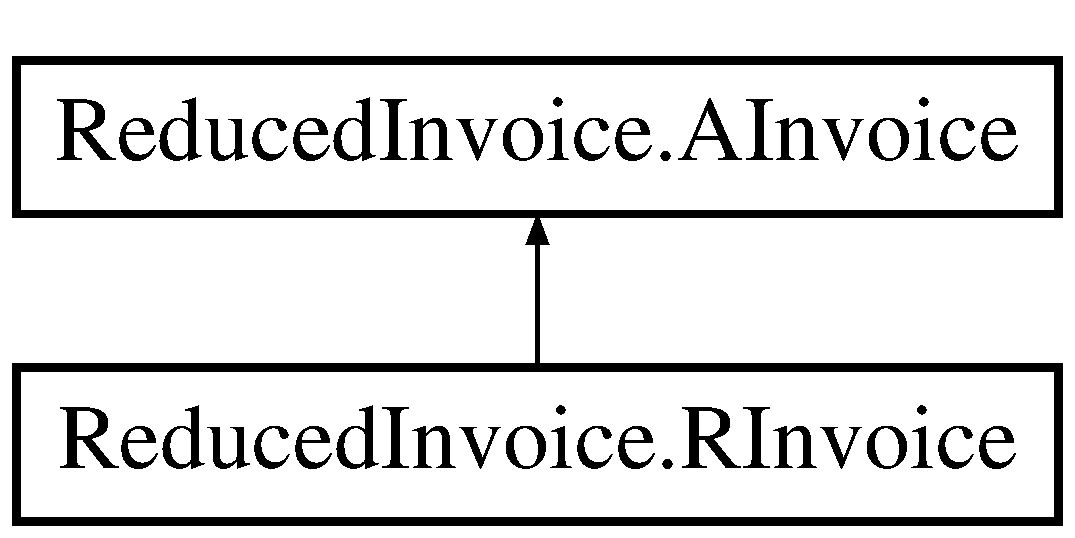
\includegraphics[height=2.000000cm]{class_reduced_invoice_1_1_r_invoice}
\end{center}
\end{figure}
\subsection*{Public Member Functions}
\begin{DoxyCompactItemize}
\item 
\hyperlink{class_reduced_invoice_1_1_r_invoice_a382c34ce7698a3e5cc9301c8cc3a5828}{R\+Invoice} ()
\item 
void \hyperlink{class_reduced_invoice_1_1_r_invoice_ae51bf96a9fc6c76ba5d79a813f4a1da0}{add\+Position} (\hyperlink{class_reduced_invoice_1_1_position}{Position} p)
\item 
void \hyperlink{class_reduced_invoice_1_1_r_invoice_aac8d8e74616bac5d81e446d47b31d5e7}{add\+Position} (String desc, \hyperlink{class_reduced_invoice_1_1_price}{Price} p, String mm, int amount, int tax)
\item 
void \hyperlink{class_reduced_invoice_1_1_r_invoice_ac851aecb0cdd4da309d203f0dfc4b55f}{add\+Position} (String desc, \hyperlink{class_reduced_invoice_1_1_price}{Price} p, String mm, int amount, int tax, \hyperlink{enum_reduced_invoice_1_1_a_invoice_1_1_error}{Error} positionerror)
\item 
\hyperlink{class_reduced_invoice_1_1_position}{Position} \hyperlink{class_reduced_invoice_1_1_r_invoice_a552d88c5808181f8fe3ca72772b5aff6}{get\+Position} (int index)
\item 
List$<$ \hyperlink{class_reduced_invoice_1_1_position}{Position} $>$ \hyperlink{class_reduced_invoice_1_1_r_invoice_a55b11262453617b33490afbc040761f6}{get\+Positions} ()
\item 
void \hyperlink{class_reduced_invoice_1_1_r_invoice_ab9c5e05457fa8a64a6ffcd8d6261e2a0}{set\+Position\+Description} (String description, int index)
\item 
void \hyperlink{class_reduced_invoice_1_1_r_invoice_a9c47d95997895b056a0e84741313dc0a}{set\+Position\+Price} (\hyperlink{class_reduced_invoice_1_1_price}{Price} price, int index)
\item 
void \hyperlink{class_reduced_invoice_1_1_r_invoice_ac463aa248993dd296ba9ea81356726b4}{set\+Position\+Amount} (int amount, int index)
\item 
void \hyperlink{class_reduced_invoice_1_1_r_invoice_a7b553ca5131f6059b022f9815be42c17}{set\+Position\+Tax\+Rate} (int taxrate, int index)
\item 
int \hyperlink{class_reduced_invoice_1_1_r_invoice_a3df22a621cc8ed79efa13bcb6284cadc}{get\+Positions\+Length} ()
\item 
void \hyperlink{class_reduced_invoice_1_1_r_invoice_a263bac524d7b762b58c124def1a20325}{set\+Position} (\hyperlink{class_reduced_invoice_1_1_position}{Position} position, int index)
\end{DoxyCompactItemize}
\subsection*{Additional Inherited Members}


\subsection{Detailed Description}


Definition at line 6 of file R\+Invoice.\+java.



\subsection{Constructor \& Destructor Documentation}
\index{Reduced\+Invoice\+::\+R\+Invoice@{Reduced\+Invoice\+::\+R\+Invoice}!R\+Invoice@{R\+Invoice}}
\index{R\+Invoice@{R\+Invoice}!Reduced\+Invoice\+::\+R\+Invoice@{Reduced\+Invoice\+::\+R\+Invoice}}
\subsubsection[{\texorpdfstring{R\+Invoice()}{RInvoice()}}]{\setlength{\rightskip}{0pt plus 5cm}Reduced\+Invoice.\+R\+Invoice.\+R\+Invoice (
\begin{DoxyParamCaption}
{}
\end{DoxyParamCaption}
)\hspace{0.3cm}{\ttfamily [inline]}}\hypertarget{class_reduced_invoice_1_1_r_invoice_a382c34ce7698a3e5cc9301c8cc3a5828}{}\label{class_reduced_invoice_1_1_r_invoice_a382c34ce7698a3e5cc9301c8cc3a5828}


Definition at line 9 of file R\+Invoice.\+java.


\begin{DoxyCode}
9                      \{
10         \hyperlink{class_reduced_invoice_1_1_a_invoice_a5b51f1865386bd021580507c7133f69a}{Positions} = \textcolor{keyword}{new} ArrayList<Position>();
11     \}
\end{DoxyCode}


\subsection{Member Function Documentation}
\index{Reduced\+Invoice\+::\+R\+Invoice@{Reduced\+Invoice\+::\+R\+Invoice}!add\+Position@{add\+Position}}
\index{add\+Position@{add\+Position}!Reduced\+Invoice\+::\+R\+Invoice@{Reduced\+Invoice\+::\+R\+Invoice}}
\subsubsection[{\texorpdfstring{add\+Position(\+Position p)}{addPosition(Position p)}}]{\setlength{\rightskip}{0pt plus 5cm}void Reduced\+Invoice.\+R\+Invoice.\+add\+Position (
\begin{DoxyParamCaption}
\item[{{\bf Position}}]{p}
\end{DoxyParamCaption}
)\hspace{0.3cm}{\ttfamily [inline]}}\hypertarget{class_reduced_invoice_1_1_r_invoice_ae51bf96a9fc6c76ba5d79a813f4a1da0}{}\label{class_reduced_invoice_1_1_r_invoice_ae51bf96a9fc6c76ba5d79a813f4a1da0}


Definition at line 14 of file R\+Invoice.\+java.


\begin{DoxyCode}
14                                         \{
15         
16         \hyperlink{class_reduced_invoice_1_1_a_invoice_a5b51f1865386bd021580507c7133f69a}{Positions}.add(p);
17     \}
\end{DoxyCode}
\index{Reduced\+Invoice\+::\+R\+Invoice@{Reduced\+Invoice\+::\+R\+Invoice}!add\+Position@{add\+Position}}
\index{add\+Position@{add\+Position}!Reduced\+Invoice\+::\+R\+Invoice@{Reduced\+Invoice\+::\+R\+Invoice}}
\subsubsection[{\texorpdfstring{add\+Position(\+String desc, Price p, String mm, int amount, int tax)}{addPosition(String desc, Price p, String mm, int amount, int tax)}}]{\setlength{\rightskip}{0pt plus 5cm}void Reduced\+Invoice.\+R\+Invoice.\+add\+Position (
\begin{DoxyParamCaption}
\item[{String}]{desc, }
\item[{{\bf Price}}]{p, }
\item[{String}]{mm, }
\item[{int}]{amount, }
\item[{int}]{tax}
\end{DoxyParamCaption}
)\hspace{0.3cm}{\ttfamily [inline]}}\hypertarget{class_reduced_invoice_1_1_r_invoice_aac8d8e74616bac5d81e446d47b31d5e7}{}\label{class_reduced_invoice_1_1_r_invoice_aac8d8e74616bac5d81e446d47b31d5e7}


Definition at line 20 of file R\+Invoice.\+java.


\begin{DoxyCode}
20                                                                                   \{
21         
22         \hyperlink{class_reduced_invoice_1_1_a_invoice_a5b51f1865386bd021580507c7133f69a}{Positions}.add(\textcolor{keyword}{new} Position(desc, p, mm, amount, tax));
23     \}
\end{DoxyCode}
\index{Reduced\+Invoice\+::\+R\+Invoice@{Reduced\+Invoice\+::\+R\+Invoice}!add\+Position@{add\+Position}}
\index{add\+Position@{add\+Position}!Reduced\+Invoice\+::\+R\+Invoice@{Reduced\+Invoice\+::\+R\+Invoice}}
\subsubsection[{\texorpdfstring{add\+Position(\+String desc, Price p, String mm, int amount, int tax, Error positionerror)}{addPosition(String desc, Price p, String mm, int amount, int tax, Error positionerror)}}]{\setlength{\rightskip}{0pt plus 5cm}void Reduced\+Invoice.\+R\+Invoice.\+add\+Position (
\begin{DoxyParamCaption}
\item[{String}]{desc, }
\item[{{\bf Price}}]{p, }
\item[{String}]{mm, }
\item[{int}]{amount, }
\item[{int}]{tax, }
\item[{{\bf Error}}]{positionerror}
\end{DoxyParamCaption}
)\hspace{0.3cm}{\ttfamily [inline]}}\hypertarget{class_reduced_invoice_1_1_r_invoice_ac851aecb0cdd4da309d203f0dfc4b55f}{}\label{class_reduced_invoice_1_1_r_invoice_ac851aecb0cdd4da309d203f0dfc4b55f}


Definition at line 26 of file R\+Invoice.\+java.


\begin{DoxyCode}
26                                                                                                        \{
27         
28         \hyperlink{class_reduced_invoice_1_1_a_invoice_a5b51f1865386bd021580507c7133f69a}{Positions}.add(\textcolor{keyword}{new} Position(desc, p, mm, amount, tax, positionerror));
29     \}
\end{DoxyCode}
\index{Reduced\+Invoice\+::\+R\+Invoice@{Reduced\+Invoice\+::\+R\+Invoice}!get\+Position@{get\+Position}}
\index{get\+Position@{get\+Position}!Reduced\+Invoice\+::\+R\+Invoice@{Reduced\+Invoice\+::\+R\+Invoice}}
\subsubsection[{\texorpdfstring{get\+Position(int index)}{getPosition(int index)}}]{\setlength{\rightskip}{0pt plus 5cm}{\bf Position} Reduced\+Invoice.\+R\+Invoice.\+get\+Position (
\begin{DoxyParamCaption}
\item[{int}]{index}
\end{DoxyParamCaption}
)\hspace{0.3cm}{\ttfamily [inline]}}\hypertarget{class_reduced_invoice_1_1_r_invoice_a552d88c5808181f8fe3ca72772b5aff6}{}\label{class_reduced_invoice_1_1_r_invoice_a552d88c5808181f8fe3ca72772b5aff6}


Definition at line 32 of file R\+Invoice.\+java.


\begin{DoxyCode}
32                                            \{
33         
34         \textcolor{keywordflow}{if}(\hyperlink{class_reduced_invoice_1_1_a_invoice_a5b51f1865386bd021580507c7133f69a}{Positions}.size() < index)
35             \textcolor{keywordflow}{return} null;
36         \textcolor{keywordflow}{else}
37             \textcolor{keywordflow}{return} \hyperlink{class_reduced_invoice_1_1_a_invoice_a5b51f1865386bd021580507c7133f69a}{Positions}.get(index);               
38     \}
\end{DoxyCode}
\index{Reduced\+Invoice\+::\+R\+Invoice@{Reduced\+Invoice\+::\+R\+Invoice}!get\+Positions@{get\+Positions}}
\index{get\+Positions@{get\+Positions}!Reduced\+Invoice\+::\+R\+Invoice@{Reduced\+Invoice\+::\+R\+Invoice}}
\subsubsection[{\texorpdfstring{get\+Positions()}{getPositions()}}]{\setlength{\rightskip}{0pt plus 5cm}List$<${\bf Position}$>$ Reduced\+Invoice.\+R\+Invoice.\+get\+Positions (
\begin{DoxyParamCaption}
{}
\end{DoxyParamCaption}
)\hspace{0.3cm}{\ttfamily [inline]}}\hypertarget{class_reduced_invoice_1_1_r_invoice_a55b11262453617b33490afbc040761f6}{}\label{class_reduced_invoice_1_1_r_invoice_a55b11262453617b33490afbc040761f6}


Definition at line 41 of file R\+Invoice.\+java.


\begin{DoxyCode}
41                                          \{
42         
43         \textcolor{keywordflow}{return} \hyperlink{class_reduced_invoice_1_1_a_invoice_a5b51f1865386bd021580507c7133f69a}{Positions};
44     \}
\end{DoxyCode}
\index{Reduced\+Invoice\+::\+R\+Invoice@{Reduced\+Invoice\+::\+R\+Invoice}!get\+Positions\+Length@{get\+Positions\+Length}}
\index{get\+Positions\+Length@{get\+Positions\+Length}!Reduced\+Invoice\+::\+R\+Invoice@{Reduced\+Invoice\+::\+R\+Invoice}}
\subsubsection[{\texorpdfstring{get\+Positions\+Length()}{getPositionsLength()}}]{\setlength{\rightskip}{0pt plus 5cm}int Reduced\+Invoice.\+R\+Invoice.\+get\+Positions\+Length (
\begin{DoxyParamCaption}
{}
\end{DoxyParamCaption}
)\hspace{0.3cm}{\ttfamily [inline]}}\hypertarget{class_reduced_invoice_1_1_r_invoice_a3df22a621cc8ed79efa13bcb6284cadc}{}\label{class_reduced_invoice_1_1_r_invoice_a3df22a621cc8ed79efa13bcb6284cadc}


Definition at line 71 of file R\+Invoice.\+java.


\begin{DoxyCode}
71                                     \{
72         
73         \textcolor{keywordflow}{return} \hyperlink{class_reduced_invoice_1_1_a_invoice_a5b51f1865386bd021580507c7133f69a}{Positions}.size();
74     \}
\end{DoxyCode}
\index{Reduced\+Invoice\+::\+R\+Invoice@{Reduced\+Invoice\+::\+R\+Invoice}!set\+Position@{set\+Position}}
\index{set\+Position@{set\+Position}!Reduced\+Invoice\+::\+R\+Invoice@{Reduced\+Invoice\+::\+R\+Invoice}}
\subsubsection[{\texorpdfstring{set\+Position(\+Position position, int index)}{setPosition(Position position, int index)}}]{\setlength{\rightskip}{0pt plus 5cm}void Reduced\+Invoice.\+R\+Invoice.\+set\+Position (
\begin{DoxyParamCaption}
\item[{{\bf Position}}]{position, }
\item[{int}]{index}
\end{DoxyParamCaption}
)\hspace{0.3cm}{\ttfamily [inline]}}\hypertarget{class_reduced_invoice_1_1_r_invoice_a263bac524d7b762b58c124def1a20325}{}\label{class_reduced_invoice_1_1_r_invoice_a263bac524d7b762b58c124def1a20325}


Definition at line 77 of file R\+Invoice.\+java.


\begin{DoxyCode}
77                                                           \{
78         
79         \hyperlink{class_reduced_invoice_1_1_a_invoice_a5b51f1865386bd021580507c7133f69a}{Positions}.get(index).setDescription(position.getDescription());
80         \hyperlink{class_reduced_invoice_1_1_a_invoice_a5b51f1865386bd021580507c7133f69a}{Positions}.get(index).setPositionPrice(position.getPositionPrice());
81         \hyperlink{class_reduced_invoice_1_1_a_invoice_a5b51f1865386bd021580507c7133f69a}{Positions}.get(index).setAmount(position.getAmount());
82         \hyperlink{class_reduced_invoice_1_1_a_invoice_a5b51f1865386bd021580507c7133f69a}{Positions}.get(index).setTaxrate(position.getTaxrate());
83     \}
\end{DoxyCode}
\index{Reduced\+Invoice\+::\+R\+Invoice@{Reduced\+Invoice\+::\+R\+Invoice}!set\+Position\+Amount@{set\+Position\+Amount}}
\index{set\+Position\+Amount@{set\+Position\+Amount}!Reduced\+Invoice\+::\+R\+Invoice@{Reduced\+Invoice\+::\+R\+Invoice}}
\subsubsection[{\texorpdfstring{set\+Position\+Amount(int amount, int index)}{setPositionAmount(int amount, int index)}}]{\setlength{\rightskip}{0pt plus 5cm}void Reduced\+Invoice.\+R\+Invoice.\+set\+Position\+Amount (
\begin{DoxyParamCaption}
\item[{int}]{amount, }
\item[{int}]{index}
\end{DoxyParamCaption}
)\hspace{0.3cm}{\ttfamily [inline]}}\hypertarget{class_reduced_invoice_1_1_r_invoice_ac463aa248993dd296ba9ea81356726b4}{}\label{class_reduced_invoice_1_1_r_invoice_ac463aa248993dd296ba9ea81356726b4}


Definition at line 59 of file R\+Invoice.\+java.


\begin{DoxyCode}
59                                                          \{
60         
61         \hyperlink{class_reduced_invoice_1_1_a_invoice_a5b51f1865386bd021580507c7133f69a}{Positions}.get(index).setAmount(amount);
62     \}
\end{DoxyCode}
\index{Reduced\+Invoice\+::\+R\+Invoice@{Reduced\+Invoice\+::\+R\+Invoice}!set\+Position\+Description@{set\+Position\+Description}}
\index{set\+Position\+Description@{set\+Position\+Description}!Reduced\+Invoice\+::\+R\+Invoice@{Reduced\+Invoice\+::\+R\+Invoice}}
\subsubsection[{\texorpdfstring{set\+Position\+Description(\+String description, int index)}{setPositionDescription(String description, int index)}}]{\setlength{\rightskip}{0pt plus 5cm}void Reduced\+Invoice.\+R\+Invoice.\+set\+Position\+Description (
\begin{DoxyParamCaption}
\item[{String}]{description, }
\item[{int}]{index}
\end{DoxyParamCaption}
)\hspace{0.3cm}{\ttfamily [inline]}}\hypertarget{class_reduced_invoice_1_1_r_invoice_ab9c5e05457fa8a64a6ffcd8d6261e2a0}{}\label{class_reduced_invoice_1_1_r_invoice_ab9c5e05457fa8a64a6ffcd8d6261e2a0}


Definition at line 47 of file R\+Invoice.\+java.


\begin{DoxyCode}
47                                                                       \{
48         
49         \hyperlink{class_reduced_invoice_1_1_a_invoice_a5b51f1865386bd021580507c7133f69a}{Positions}.get(index).setDescription(description);
50     \}
\end{DoxyCode}
\index{Reduced\+Invoice\+::\+R\+Invoice@{Reduced\+Invoice\+::\+R\+Invoice}!set\+Position\+Price@{set\+Position\+Price}}
\index{set\+Position\+Price@{set\+Position\+Price}!Reduced\+Invoice\+::\+R\+Invoice@{Reduced\+Invoice\+::\+R\+Invoice}}
\subsubsection[{\texorpdfstring{set\+Position\+Price(\+Price price, int index)}{setPositionPrice(Price price, int index)}}]{\setlength{\rightskip}{0pt plus 5cm}void Reduced\+Invoice.\+R\+Invoice.\+set\+Position\+Price (
\begin{DoxyParamCaption}
\item[{{\bf Price}}]{price, }
\item[{int}]{index}
\end{DoxyParamCaption}
)\hspace{0.3cm}{\ttfamily [inline]}}\hypertarget{class_reduced_invoice_1_1_r_invoice_a9c47d95997895b056a0e84741313dc0a}{}\label{class_reduced_invoice_1_1_r_invoice_a9c47d95997895b056a0e84741313dc0a}


Definition at line 53 of file R\+Invoice.\+java.


\begin{DoxyCode}
53                                                          \{
54         
55         \hyperlink{class_reduced_invoice_1_1_a_invoice_a5b51f1865386bd021580507c7133f69a}{Positions}.get(index).setPositionPrice(price);
56     \}
\end{DoxyCode}
\index{Reduced\+Invoice\+::\+R\+Invoice@{Reduced\+Invoice\+::\+R\+Invoice}!set\+Position\+Tax\+Rate@{set\+Position\+Tax\+Rate}}
\index{set\+Position\+Tax\+Rate@{set\+Position\+Tax\+Rate}!Reduced\+Invoice\+::\+R\+Invoice@{Reduced\+Invoice\+::\+R\+Invoice}}
\subsubsection[{\texorpdfstring{set\+Position\+Tax\+Rate(int taxrate, int index)}{setPositionTaxRate(int taxrate, int index)}}]{\setlength{\rightskip}{0pt plus 5cm}void Reduced\+Invoice.\+R\+Invoice.\+set\+Position\+Tax\+Rate (
\begin{DoxyParamCaption}
\item[{int}]{taxrate, }
\item[{int}]{index}
\end{DoxyParamCaption}
)\hspace{0.3cm}{\ttfamily [inline]}}\hypertarget{class_reduced_invoice_1_1_r_invoice_a7b553ca5131f6059b022f9815be42c17}{}\label{class_reduced_invoice_1_1_r_invoice_a7b553ca5131f6059b022f9815be42c17}


Definition at line 65 of file R\+Invoice.\+java.


\begin{DoxyCode}
65                                                            \{
66 
67         \hyperlink{class_reduced_invoice_1_1_a_invoice_a5b51f1865386bd021580507c7133f69a}{Positions}.get(index).setTaxrate(taxrate);
68     \}
\end{DoxyCode}


The documentation for this class was generated from the following file\+:\begin{DoxyCompactItemize}
\item 
C\+:/\+Users/\+Denis/workspace/taxsynapse/src/main/java/\+Reduced\+Invoice/\hyperlink{_r_invoice_8java}{R\+Invoice.\+java}\end{DoxyCompactItemize}

\hypertarget{class_application_1_1_run}{}\section{Application.\+Run Class Reference}
\label{class_application_1_1_run}\index{Application.\+Run@{Application.\+Run}}
\subsection*{Static Public Member Functions}
\begin{DoxyCompactItemize}
\item 
static void \hyperlink{class_application_1_1_run_a57a17174b40d7c0feba22e460fa6158c}{main} (String\mbox{[}$\,$\mbox{]} args)  throws I\+O\+Exception 
\end{DoxyCompactItemize}


\subsection{Detailed Description}


Definition at line 11 of file Run.\+java.



\subsection{Member Function Documentation}
\index{Application\+::\+Run@{Application\+::\+Run}!main@{main}}
\index{main@{main}!Application\+::\+Run@{Application\+::\+Run}}
\subsubsection[{\texorpdfstring{main(\+String[] args)}{main(String[] args)}}]{\setlength{\rightskip}{0pt plus 5cm}static void Application.\+Run.\+main (
\begin{DoxyParamCaption}
\item[{String\mbox{[}$\,$\mbox{]}}]{args}
\end{DoxyParamCaption}
) throws I\+O\+Exception\hspace{0.3cm}{\ttfamily [inline]}, {\ttfamily [static]}}\hypertarget{class_application_1_1_run_a57a17174b40d7c0feba22e460fa6158c}{}\label{class_application_1_1_run_a57a17174b40d7c0feba22e460fa6158c}
Override Validation Counter

Serialization 

Definition at line 21 of file Run.\+java.


\begin{DoxyCode}
21                                                               \{
22         
23         String pathToFolder = args[0];
24         Boolean logSingleSteps = Boolean.valueOf(args[1]);
25         Boolean supressInvalid = Boolean.valueOf(args[2]);
26         
27         \hyperlink{class_import_1_1zugferd_handler}{zugferdHandler} zHandler = \hyperlink{class_import_1_1zugferd_handler}{zugferdHandler}.
      \hyperlink{class_import_1_1zugferd_handler_ad3acd84340c8a5fcb2c01a2636979786}{getInstance}();
28         List<Invoice> InvoiceList = \textcolor{keyword}{new} ArrayList<Invoice>();
29         List<AInvoice> ReducedInvoiceList = \textcolor{keyword}{new} ArrayList<AInvoice>();
30         
31         System.out.println(\textcolor{stringliteral}{"Please ignore log4j Warnings"});
32         \textcolor{comment}{//Read Invoices from Folder and add to List}
33         \textcolor{keywordflow}{try}\{
34             zHandler.\hyperlink{class_import_1_1zugferd_handler_aea79c23595f003c943e908c95276ecf9}{readInvoice}(pathToFolder, InvoiceList, logSingleSteps, supressInvalid);
35             System.out.println(\textcolor{stringliteral}{"All Invoices successfully readed"});
36             \hyperlink{class_reduced_invoice_1_1_invoice_reducer}{InvoiceReducer} ir = \hyperlink{class_reduced_invoice_1_1_invoice_reducer}{InvoiceReducer}.
      \hyperlink{class_reduced_invoice_1_1_invoice_reducer_ad4fafc7b331a78ef243c3e3ba88803da}{getInstance}();
37             ir.\hyperlink{class_reduced_invoice_1_1_invoice_reducer_af064188d62db15e810468e4811af6cc5}{ReducedInvoiceList}(InvoiceList, ReducedInvoiceList);
38             System.out.println(\textcolor{stringliteral}{"Successfully reduced Invoices"});
39             System.out.println(\textcolor{stringliteral}{"MetaExceptionCounter: "} + ir.
      \hyperlink{class_reduced_invoice_1_1_invoice_reducer_a987de6f3876284a7b456240f85dc066f}{getMetaExceptionCounter}());
40             System.out.println(\textcolor{stringliteral}{"PositionExceptionCounter: "} + ir.
      \hyperlink{class_reduced_invoice_1_1_invoice_reducer_ad5034d72d8eae0edc2026c9ca9e66465}{getPositionExceptionCounter}());
41             
42             
43         \}\textcolor{keywordflow}{catch}(Exception e)\{
44             System.out.print(\textcolor{stringliteral}{"Exception while reducing Invoices"});
45             System.out.println(\textcolor{stringliteral}{"Details: "});
46             System.out.println(e.getMessage());
47         \}
48         
49         System.out.println(\textcolor{stringliteral}{"Breakpoint"});
50         
51     \}
\end{DoxyCode}


The documentation for this class was generated from the following file\+:\begin{DoxyCompactItemize}
\item 
C\+:/\+Users/\+Denis/workspace/taxsynapse/src/main/java/\+Application/\hyperlink{_run_8java}{Run.\+java}\end{DoxyCompactItemize}

\hypertarget{class_import_1_1zugferd_handler}{\section{Import.\-zugferd\-Handler Class Reference}
\label{class_import_1_1zugferd_handler}\index{Import.\-zugferd\-Handler@{Import.\-zugferd\-Handler}}
}
\subsection*{Public Member Functions}
\begin{DoxyCompactItemize}
\item 
Invoice \hyperlink{class_import_1_1zugferd_handler_aea79c23595f003c943e908c95276ecf9}{read\-Invoice} (String Path)  throws I\-O\-Exception
\item 
void \hyperlink{class_import_1_1zugferd_handler_a693fba6ff3bd23bb4783578b385e38a4}{read\-Invoice} (String Path, List$<$ \hyperlink{class_reduced_invoice_1_1_a_invoice}{A\-Invoice} $>$ Reduced\-Invoice\-List, final boolean set\-Logging, final boolean supress\-Invalid)  throws Exception 	
\item 
void \hyperlink{class_import_1_1zugferd_handler_aa5fbab8b4a7835f2b13167452f9d17db}{remove\-Invalid} (List$<$ Invoice $>$ Invoice\-List)
\item 
boolean \hyperlink{class_import_1_1zugferd_handler_a6999d186193b120650a5d24a49d10c6c}{has\-Invalid} (List$<$ Invoice $>$ Invoice\-List)
\item 
Set$<$ Constraint\-Violation\\*
$<$ Invoice $>$ $>$ \hyperlink{class_import_1_1zugferd_handler_acf26740b73f820812fadb01ccf712dd2}{get\-Violations} (Invoice invoice)
\item 
void \hyperlink{class_import_1_1zugferd_handler_ae8ae1fcc05ebddf4d2b53c8daeda7b00}{print\-Violations} (List$<$ Invoice $>$ Invoice\-List)
\item 
void \hyperlink{class_import_1_1zugferd_handler_aadb33b773805373add19d92eb713831b}{print\-Single\-Invoice\-Violations} (Invoice invoice)
\end{DoxyCompactItemize}
\subsection*{Static Public Member Functions}
\begin{DoxyCompactItemize}
\item 
static \hyperlink{class_import_1_1zugferd_handler}{zugferd\-Handler} \hyperlink{class_import_1_1zugferd_handler_ad3acd84340c8a5fcb2c01a2636979786}{get\-Instance} ()
\end{DoxyCompactItemize}


\subsection{Detailed Description}


Definition at line 23 of file zugferd\-Handler.\-java.



\subsection{Member Function Documentation}
\hypertarget{class_import_1_1zugferd_handler_ad3acd84340c8a5fcb2c01a2636979786}{\index{Import\-::zugferd\-Handler@{Import\-::zugferd\-Handler}!get\-Instance@{get\-Instance}}
\index{get\-Instance@{get\-Instance}!Import::zugferdHandler@{Import\-::zugferd\-Handler}}
\subsubsection[{get\-Instance}]{\setlength{\rightskip}{0pt plus 5cm}static {\bf zugferd\-Handler} Import.\-zugferd\-Handler.\-get\-Instance (
\begin{DoxyParamCaption}
{}
\end{DoxyParamCaption}
)\hspace{0.3cm}{\ttfamily [inline]}, {\ttfamily [static]}}}\label{class_import_1_1zugferd_handler_ad3acd84340c8a5fcb2c01a2636979786}


Definition at line 29 of file zugferd\-Handler.\-java.


\begin{DoxyCode}
29                                               \{
30         \textcolor{keywordflow}{if}(uniqueInstance == null) \{
31             \textcolor{keyword}{synchronized}(zugferdHandler.class)\{
32                 \textcolor{keywordflow}{if}(uniqueInstance == null)\{
33                     uniqueInstance = \textcolor{keyword}{new} zugferdHandler();
34                 \}
35             \}
36         \}
37         \textcolor{keywordflow}{return} uniqueInstance;
38     \}
\end{DoxyCode}
\hypertarget{class_import_1_1zugferd_handler_acf26740b73f820812fadb01ccf712dd2}{\index{Import\-::zugferd\-Handler@{Import\-::zugferd\-Handler}!get\-Violations@{get\-Violations}}
\index{get\-Violations@{get\-Violations}!Import::zugferdHandler@{Import\-::zugferd\-Handler}}
\subsubsection[{get\-Violations}]{\setlength{\rightskip}{0pt plus 5cm}Set$<$Constraint\-Violation$<$Invoice$>$ $>$ Import.\-zugferd\-Handler.\-get\-Violations (
\begin{DoxyParamCaption}
\item[{Invoice}]{invoice}
\end{DoxyParamCaption}
)\hspace{0.3cm}{\ttfamily [inline]}}}\label{class_import_1_1zugferd_handler_acf26740b73f820812fadb01ccf712dd2}


Definition at line 131 of file zugferd\-Handler.\-java.


\begin{DoxyCode}
131                                                                             \{
132         
133         InvoiceValidator invoiceValidator = \textcolor{keyword}{new} InvoiceValidator();
134        
135         Set<ConstraintViolation<Invoice>> violations = invoiceValidator.validate(invoice);
136         
137         \textcolor{keywordflow}{return} violations;
138     \}
\end{DoxyCode}
\hypertarget{class_import_1_1zugferd_handler_a6999d186193b120650a5d24a49d10c6c}{\index{Import\-::zugferd\-Handler@{Import\-::zugferd\-Handler}!has\-Invalid@{has\-Invalid}}
\index{has\-Invalid@{has\-Invalid}!Import::zugferdHandler@{Import\-::zugferd\-Handler}}
\subsubsection[{has\-Invalid}]{\setlength{\rightskip}{0pt plus 5cm}boolean Import.\-zugferd\-Handler.\-has\-Invalid (
\begin{DoxyParamCaption}
\item[{List$<$ Invoice $>$}]{Invoice\-List}
\end{DoxyParamCaption}
)\hspace{0.3cm}{\ttfamily [inline]}}}\label{class_import_1_1zugferd_handler_a6999d186193b120650a5d24a49d10c6c}


Definition at line 122 of file zugferd\-Handler.\-java.


\begin{DoxyCode}
122                                                         \{
123         
124         \textcolor{keywordflow}{for} (Invoice temp : InvoiceList) \{
125             \textcolor{keywordflow}{if}(this.\hyperlink{class_import_1_1zugferd_handler_acf26740b73f820812fadb01ccf712dd2}{getViolations}(temp) != null)
126                 \textcolor{keywordflow}{return} \textcolor{keyword}{true};
127         \}
128         \textcolor{keywordflow}{return} \textcolor{keyword}{false};
129     \}
\end{DoxyCode}
\hypertarget{class_import_1_1zugferd_handler_aadb33b773805373add19d92eb713831b}{\index{Import\-::zugferd\-Handler@{Import\-::zugferd\-Handler}!print\-Single\-Invoice\-Violations@{print\-Single\-Invoice\-Violations}}
\index{print\-Single\-Invoice\-Violations@{print\-Single\-Invoice\-Violations}!Import::zugferdHandler@{Import\-::zugferd\-Handler}}
\subsubsection[{print\-Single\-Invoice\-Violations}]{\setlength{\rightskip}{0pt plus 5cm}void Import.\-zugferd\-Handler.\-print\-Single\-Invoice\-Violations (
\begin{DoxyParamCaption}
\item[{Invoice}]{invoice}
\end{DoxyParamCaption}
)\hspace{0.3cm}{\ttfamily [inline]}}}\label{class_import_1_1zugferd_handler_aadb33b773805373add19d92eb713831b}


Definition at line 154 of file zugferd\-Handler.\-java.


\begin{DoxyCode}
154                                                              \{
155         
156         InvoiceValidator invoiceValidator = \textcolor{keyword}{new} InvoiceValidator();
157         
158         Set<ConstraintViolation<Invoice>> violations = invoiceValidator.validate(invoice);
159         
160         \textcolor{keywordflow}{for} (ConstraintViolation<Invoice> violation : violations) \{
161              System.out.println((violation.getMessage() + \textcolor{stringliteral}{" at: "} + violation.getPropertyPath()));
162            \}
163     \}
\end{DoxyCode}
\hypertarget{class_import_1_1zugferd_handler_ae8ae1fcc05ebddf4d2b53c8daeda7b00}{\index{Import\-::zugferd\-Handler@{Import\-::zugferd\-Handler}!print\-Violations@{print\-Violations}}
\index{print\-Violations@{print\-Violations}!Import::zugferdHandler@{Import\-::zugferd\-Handler}}
\subsubsection[{print\-Violations}]{\setlength{\rightskip}{0pt plus 5cm}void Import.\-zugferd\-Handler.\-print\-Violations (
\begin{DoxyParamCaption}
\item[{List$<$ Invoice $>$}]{Invoice\-List}
\end{DoxyParamCaption}
)\hspace{0.3cm}{\ttfamily [inline]}}}\label{class_import_1_1zugferd_handler_ae8ae1fcc05ebddf4d2b53c8daeda7b00}


Definition at line 140 of file zugferd\-Handler.\-java.


\begin{DoxyCode}
140                                                           \{
141         
142         InvoiceValidator invoiceValidator = \textcolor{keyword}{new} InvoiceValidator();
143         
144         Set<ConstraintViolation<Invoice>> violations;
145         
146         \textcolor{keywordflow}{for} (Invoice temp : InvoiceList) \{
147             violations = invoiceValidator.validate(temp);
148             \textcolor{keywordflow}{for} (ConstraintViolation<Invoice> violation : violations) \{
149                  System.out.println((violation.getMessage() + \textcolor{stringliteral}{" at: "} + violation.getPropertyPath()));
150             \}
151         \}
152     \}
\end{DoxyCode}
\hypertarget{class_import_1_1zugferd_handler_aea79c23595f003c943e908c95276ecf9}{\index{Import\-::zugferd\-Handler@{Import\-::zugferd\-Handler}!read\-Invoice@{read\-Invoice}}
\index{read\-Invoice@{read\-Invoice}!Import::zugferdHandler@{Import\-::zugferd\-Handler}}
\subsubsection[{read\-Invoice}]{\setlength{\rightskip}{0pt plus 5cm}Invoice Import.\-zugferd\-Handler.\-read\-Invoice (
\begin{DoxyParamCaption}
\item[{String}]{Path}
\end{DoxyParamCaption}
) throws I\-O\-Exception\hspace{0.3cm}{\ttfamily [inline]}}}\label{class_import_1_1zugferd_handler_aea79c23595f003c943e908c95276ecf9}


Definition at line 40 of file zugferd\-Handler.\-java.


\begin{DoxyCode}
40                                                               \{
41         
42         PdfHandler handler = \textcolor{keyword}{new} PdfHandler();
43         
44         FileInputStream input = \textcolor{keyword}{new} FileInputStream(\textcolor{keyword}{new} File(Path));
45         
46         Invoice invoice = handler.extractInvoice(input);
47         
48         \textcolor{keywordflow}{if}(invoice != null)
49             \textcolor{keywordflow}{return} invoice;
50         \textcolor{keywordflow}{else}
51             \textcolor{keywordflow}{return} null;
52     \}
\end{DoxyCode}
\hypertarget{class_import_1_1zugferd_handler_a693fba6ff3bd23bb4783578b385e38a4}{\index{Import\-::zugferd\-Handler@{Import\-::zugferd\-Handler}!read\-Invoice@{read\-Invoice}}
\index{read\-Invoice@{read\-Invoice}!Import::zugferdHandler@{Import\-::zugferd\-Handler}}
\subsubsection[{read\-Invoice}]{\setlength{\rightskip}{0pt plus 5cm}void Import.\-zugferd\-Handler.\-read\-Invoice (
\begin{DoxyParamCaption}
\item[{String}]{Path, }
\item[{List$<$ {\bf A\-Invoice} $>$}]{Reduced\-Invoice\-List, }
\item[{final boolean}]{set\-Logging, }
\item[{final boolean}]{supress\-Invalid}
\end{DoxyParamCaption}
) throws Exception\hspace{0.3cm}{\ttfamily [inline]}}}\label{class_import_1_1zugferd_handler_a693fba6ff3bd23bb4783578b385e38a4}


Definition at line 54 of file zugferd\-Handler.\-java.


\begin{DoxyCode}
55     \{
56         InvoiceReducer ir = InvoiceReducer.getInstance();
57         \textcolor{comment}{//Rekursive => elem can be a folder or a file }
58         Files.walk(Paths.get(Path)).forEach(elem -> \{
59             String fileName = elem.getFileName().toString();
60             String path = elem.toString();
61             \textcolor{keywordflow}{try}\{
62                 \textcolor{keywordflow}{if} (Files.isDirectory(elem))\{
63                     \textcolor{keywordflow}{if}(setLogging)\{ System.out.println(\textcolor{stringliteral}{"recursive entry. elem is just a directory."}); \}
64                 \}\textcolor{keywordflow}{else}\{  \textcolor{keywordflow}{if}(Files.isRegularFile(elem))\{
65                     \textcolor{keywordflow}{if}(Files.probeContentType(elem).intern() == \textcolor{stringliteral}{"application/pdf"})\{
66                         Invoice invoice = this.readInvoice(path);
67                         \textcolor{keywordflow}{if}(invoice != null) \{
68                             \textcolor{keywordtype}{boolean} add = \textcolor{keyword}{false};
69                             \textcolor{keywordflow}{if}(supressInvalid)\{
70                                 Set<ConstraintViolation<Invoice>> violations = this.getViolations(invoice);
71                                 \textcolor{keywordflow}{if}((violations.size() > 0))\{
72                                     \textcolor{keywordflow}{if}(setLogging)\{ System.out.println(\textcolor{stringliteral}{"Violatins found in: "} + fileName); 
      \}
73                                     \textcolor{keywordflow}{if}(setLogging)\{ 
74                                         violations.forEach(vio -> \{
75                                             System.out.println(vio.getExecutableReturnValue() + \textcolor{stringliteral}{"|"} + vio.
      getLeafBean() + \textcolor{stringliteral}{"|"} + vio.getInvalidValue() + \textcolor{stringliteral}{"|"} + vio.getMessage());
76                                         \});
77                                     \}
78                                     add = \textcolor{keyword}{false};
79                                 \}\textcolor{keywordflow}{else}\{
80                                     add = \textcolor{keyword}{true};
81                                 \}
82                             \}\textcolor{keywordflow}{else}\{
83                                 add = \textcolor{keyword}{true};
84                             \}
85                             \textcolor{keywordflow}{if}(add)\{
86                                 \textcolor{keywordflow}{if}(setLogging)\{ System.out.println(fileName + \textcolor{stringliteral}{" is valid."} ); \}
87                                 ReducedInvoiceList.add(ir.ConvertInvoiceToRinvoice(invoice, fileName));
88                                 \textcolor{keywordflow}{if}(setLogging)\{ System.out.println( fileName + \textcolor{stringliteral}{" added to the list."}); \}
89                             \}
90                         \}
91                     \}\textcolor{keywordflow}{else}\{
92                         \textcolor{keywordflow}{if}(setLogging)\{ System.out.println(\textcolor{stringliteral}{"a non pdf file was found. Ignoring..."}); \}
93                     \}
94                 \}\textcolor{keywordflow}{else}\{
95                     \textcolor{keywordflow}{if}(setLogging)\{ System.out.println(\textcolor{stringliteral}{"elem is neither a directory nor a file. Ignoring...
      "}); \}
96                 \}\}
97             \}\textcolor{keywordflow}{catch}(TransformationException tfe)\{
98                 \textcolor{keywordflow}{if}(setLogging)\{ 
99                     System.out.println(fileName + \textcolor{stringliteral}{" caused an Exception while transforming PDF/ZUGFERD to
       Java/Invoice"});
100                     System.out.println(\textcolor{stringliteral}{"Message: "} + tfe.getMessage());
101                 \}
102             \}\textcolor{keywordflow}{catch}(IOException ioe)\{
103                 \textcolor{keywordflow}{if}(setLogging)\{ 
104                     System.out.println(fileName + \textcolor{stringliteral}{" caused an IOException."});
105                     System.out.println(\textcolor{stringliteral}{"Message: "} + ioe.getMessage());
106                 \}
107             \}\textcolor{keywordflow}{catch}(Exception e)\{
108                 \textcolor{keywordflow}{if}(setLogging)\{ 
109                     System.out.println(fileName + \textcolor{stringliteral}{" caused an Exception."});
110                     System.out.println(\textcolor{stringliteral}{"Message: "} + e.getMessage());
111                 \}
112             \}
113         \});
114     \}
\end{DoxyCode}
\hypertarget{class_import_1_1zugferd_handler_aa5fbab8b4a7835f2b13167452f9d17db}{\index{Import\-::zugferd\-Handler@{Import\-::zugferd\-Handler}!remove\-Invalid@{remove\-Invalid}}
\index{remove\-Invalid@{remove\-Invalid}!Import::zugferdHandler@{Import\-::zugferd\-Handler}}
\subsubsection[{remove\-Invalid}]{\setlength{\rightskip}{0pt plus 5cm}void Import.\-zugferd\-Handler.\-remove\-Invalid (
\begin{DoxyParamCaption}
\item[{List$<$ Invoice $>$}]{Invoice\-List}
\end{DoxyParamCaption}
)\hspace{0.3cm}{\ttfamily [inline]}}}\label{class_import_1_1zugferd_handler_aa5fbab8b4a7835f2b13167452f9d17db}


Definition at line 117 of file zugferd\-Handler.\-java.


\begin{DoxyCode}
117                                                         \{
118         
119         InvoiceList.removeIf(i -> \hyperlink{class_import_1_1zugferd_handler_acf26740b73f820812fadb01ccf712dd2}{getViolations}(i).size() <= 0);
120     \}
\end{DoxyCode}


The documentation for this class was generated from the following file\-:\begin{DoxyCompactItemize}
\item 
H\-:/\-Programmierungen/\-Java/taxsynapse/src/main/java/\-Import/\hyperlink{zugferd_handler_8java}{zugferd\-Handler.\-java}\end{DoxyCompactItemize}

\chapter{File Documentation}
\hypertarget{_run_8java}{}\section{C\+:/\+Users/\+Denis/workspace/taxsynapse/src/main/java/\+Application/\+Run.java File Reference}
\label{_run_8java}\index{C\+:/\+Users/\+Denis/workspace/taxsynapse/src/main/java/\+Application/\+Run.\+java@{C\+:/\+Users/\+Denis/workspace/taxsynapse/src/main/java/\+Application/\+Run.\+java}}
\subsection*{Classes}
\begin{DoxyCompactItemize}
\item 
class \hyperlink{class_application_1_1_run}{Application.\+Run}
\end{DoxyCompactItemize}
\subsection*{Packages}
\begin{DoxyCompactItemize}
\item 
package \hyperlink{namespace_application}{Application}
\end{DoxyCompactItemize}

\hypertarget{zugferd_handler_8java}{\section{H\-:/\-Programmierungen/\-Java/taxsynapse/src/main/java/\-Import/zugferd\-Handler.java File Reference}
\label{zugferd_handler_8java}\index{H\-:/\-Programmierungen/\-Java/taxsynapse/src/main/java/\-Import/zugferd\-Handler.\-java@{H\-:/\-Programmierungen/\-Java/taxsynapse/src/main/java/\-Import/zugferd\-Handler.\-java}}
}
\subsection*{Classes}
\begin{DoxyCompactItemize}
\item 
class \hyperlink{class_import_1_1zugferd_handler}{Import.\-zugferd\-Handler}
\end{DoxyCompactItemize}
\subsection*{Packages}
\begin{DoxyCompactItemize}
\item 
package \hyperlink{namespace_import}{Import}
\end{DoxyCompactItemize}

\hypertarget{_a_invoice_8java}{\section{H\-:/\-Programmierungen/\-Java/taxsynapse/src/main/java/\-Reduced\-Invoice/\-A\-Invoice.java File Reference}
\label{_a_invoice_8java}\index{H\-:/\-Programmierungen/\-Java/taxsynapse/src/main/java/\-Reduced\-Invoice/\-A\-Invoice.\-java@{H\-:/\-Programmierungen/\-Java/taxsynapse/src/main/java/\-Reduced\-Invoice/\-A\-Invoice.\-java}}
}
\subsection*{Classes}
\begin{DoxyCompactItemize}
\item 
class \hyperlink{class_reduced_invoice_1_1_a_invoice}{Reduced\-Invoice.\-A\-Invoice}
\item 
enum \hyperlink{enum_reduced_invoice_1_1_a_invoice_1_1_error}{Reduced\-Invoice.\-A\-Invoice.\-Error}
\end{DoxyCompactItemize}
\subsection*{Packages}
\begin{DoxyCompactItemize}
\item 
package \hyperlink{namespace_reduced_invoice}{Reduced\-Invoice}
\end{DoxyCompactItemize}

\hypertarget{_invoice_reducer_8java}{\section{H\-:/\-Programmierungen/\-Java/taxsynapse/src/main/java/\-Reduced\-Invoice/\-Invoice\-Reducer.java File Reference}
\label{_invoice_reducer_8java}\index{H\-:/\-Programmierungen/\-Java/taxsynapse/src/main/java/\-Reduced\-Invoice/\-Invoice\-Reducer.\-java@{H\-:/\-Programmierungen/\-Java/taxsynapse/src/main/java/\-Reduced\-Invoice/\-Invoice\-Reducer.\-java}}
}
\subsection*{Classes}
\begin{DoxyCompactItemize}
\item 
class \hyperlink{class_reduced_invoice_1_1_invoice_reducer}{Reduced\-Invoice.\-Invoice\-Reducer}
\end{DoxyCompactItemize}
\subsection*{Packages}
\begin{DoxyCompactItemize}
\item 
package \hyperlink{namespace_reduced_invoice}{Reduced\-Invoice}
\end{DoxyCompactItemize}

\hypertarget{_metadata_8java}{}\section{C\+:/\+Users/\+Denis/workspace/taxsynapse/src/main/java/\+Reduced\+Invoice/\+Metadata.java File Reference}
\label{_metadata_8java}\index{C\+:/\+Users/\+Denis/workspace/taxsynapse/src/main/java/\+Reduced\+Invoice/\+Metadata.\+java@{C\+:/\+Users/\+Denis/workspace/taxsynapse/src/main/java/\+Reduced\+Invoice/\+Metadata.\+java}}
\subsection*{Classes}
\begin{DoxyCompactItemize}
\item 
class \hyperlink{class_reduced_invoice_1_1_metadata}{Reduced\+Invoice.\+Metadata}
\end{DoxyCompactItemize}
\subsection*{Packages}
\begin{DoxyCompactItemize}
\item 
package \hyperlink{namespace_reduced_invoice}{Reduced\+Invoice}
\end{DoxyCompactItemize}

\hypertarget{_position_8java}{}\section{C\+:/\+Users/\+Denis/workspace/taxsynapse/src/main/java/\+Reduced\+Invoice/\+Position.java File Reference}
\label{_position_8java}\index{C\+:/\+Users/\+Denis/workspace/taxsynapse/src/main/java/\+Reduced\+Invoice/\+Position.\+java@{C\+:/\+Users/\+Denis/workspace/taxsynapse/src/main/java/\+Reduced\+Invoice/\+Position.\+java}}
\subsection*{Classes}
\begin{DoxyCompactItemize}
\item 
class \hyperlink{class_reduced_invoice_1_1_position}{Reduced\+Invoice.\+Position}
\end{DoxyCompactItemize}
\subsection*{Packages}
\begin{DoxyCompactItemize}
\item 
package \hyperlink{namespace_reduced_invoice}{Reduced\+Invoice}
\end{DoxyCompactItemize}

\hypertarget{_price_8java}{}\section{C\+:/\+Users/\+Denis/workspace/taxsynapse/src/main/java/\+Reduced\+Invoice/\+Price.java File Reference}
\label{_price_8java}\index{C\+:/\+Users/\+Denis/workspace/taxsynapse/src/main/java/\+Reduced\+Invoice/\+Price.\+java@{C\+:/\+Users/\+Denis/workspace/taxsynapse/src/main/java/\+Reduced\+Invoice/\+Price.\+java}}
\subsection*{Classes}
\begin{DoxyCompactItemize}
\item 
class \hyperlink{class_reduced_invoice_1_1_price}{Reduced\+Invoice.\+Price}
\end{DoxyCompactItemize}
\subsection*{Packages}
\begin{DoxyCompactItemize}
\item 
package \hyperlink{namespace_reduced_invoice}{Reduced\+Invoice}
\end{DoxyCompactItemize}

\hypertarget{_r_invoice_8java}{\section{H\-:/\-Programmierungen/\-Java/taxsynapse/src/main/java/\-Reduced\-Invoice/\-R\-Invoice.java File Reference}
\label{_r_invoice_8java}\index{H\-:/\-Programmierungen/\-Java/taxsynapse/src/main/java/\-Reduced\-Invoice/\-R\-Invoice.\-java@{H\-:/\-Programmierungen/\-Java/taxsynapse/src/main/java/\-Reduced\-Invoice/\-R\-Invoice.\-java}}
}
\subsection*{Classes}
\begin{DoxyCompactItemize}
\item 
class \hyperlink{class_reduced_invoice_1_1_r_invoice}{Reduced\-Invoice.\-R\-Invoice}
\end{DoxyCompactItemize}
\subsection*{Packages}
\begin{DoxyCompactItemize}
\item 
package \hyperlink{namespace_reduced_invoice}{Reduced\-Invoice}
\end{DoxyCompactItemize}

\hypertarget{mainpage_8txt}{\section{mainpage.\-txt File Reference}
\label{mainpage_8txt}\index{mainpage.\-txt@{mainpage.\-txt}}
}

%--- End generated contents ---

% Index
\backmatter
\newpage
\phantomsection
\clearemptydoublepage
\addcontentsline{toc}{chapter}{Index}
\printindex

\end{document}
